\documentclass{article}
\usepackage{amsmath}
\usepackage{amssymb}
\usepackage{amsthm}

% Operators
\newcommand{\diag}{\operatorname{diag}}
\newcommand{\Hom}{\operatorname{Hom}}
\newcommand{\Rep}{\operatorname{Rep}}
\newcommand{\rank}{\operatorname{rank}}
\newcommand{\Supp}{\operatorname{Supp}}
\usepackage{graphicx}
\usepackage{geometry}
\usepackage{graphicx}
\usepackage{hyperref}
% Required packages for algorithms
\usepackage{algorithm}
\usepackage{algpseudocode}
\usepackage{subcaption}
\usepackage[normalem]{ulem}
\usepackage{comment}
\usepackage{tikz}
\usetikzlibrary{arrows.meta,positioning}
% theorem/proposition environments
\theoremstyle{definition}
\newtheorem{theorem}{Theorem}[section]
\newtheorem{proposition}[theorem]{Proposition}
\newtheorem{lemma}[theorem]{Lemma}
\newtheorem{corollary}[theorem]{Corollary}
\newtheorem{definition}[theorem]{Definition}
\newtheorem{remark}[theorem]{Remark}
\title{Notes on the Geometry of Deep Linear Networks}
\begin{document}
\maketitle
\section{Deep Linear Networks}\label{sec:dln}
\begin{definition}\label{def:dln}
    A deep linear network (DLN) is parameter-function map defined by a composition of linear transformations. For input space $\mathbb{R}^{d_0}$, output space $\mathbb{R}^{d_L}$, and $L$ layers with weight matrices $W_1 \in \mathbb{R}^{d_1 \times d_0}, W_2 \in \mathbb{R}^{d_2 \times d_1}, \ldots, W_L \in \mathbb{R}^{d_L \times d_{L-1}}$, the DLN is given by:
    \begin{equation*}
        f(x; W_1, W_2, \ldots, W_L) = W_L W_{L-1} \cdots W_1 x,
    \end{equation*}
    where $x \in \mathbb{R}^{d_0}$ is an input vector.
\end{definition}
Note that the DLN $f$ is a polynomial function of the entries of the weight matrices and linear in the input $x$.
\begin{lemma}\label{lem:parameter-manifold}
    The space of parameter $\Omega = $$\mathbb{R}^{d_1 \times d_0} \times \mathbb{R}^{d_2 \times d_1} \times \cdots \times \mathbb{R}^{d_L \times d_{L-1}}$ is a a differentiable manifold of dimension $\sum_{l=1}^L d_l d_{l-1}$. Furthermore, the space $\Omega$ has a scalar product:
    \begin{equation*}
        \langle U, V \rangle := \sum_{l=1}^L \langle U_l, V_l \rangle_F = \sum_{l=1}^L \text{Tr}(U_l^{\top} V_l)
    \end{equation*}
\end{lemma}
 The differential is induced by the differential on the Euclidean spaces $\mathbb{R}^{d_l \times d_{l-1}}$. The scalar product is induced by the Frobenius scalar product on each of the Euclidean spaces $\mathbb{R}^{d_l \times d_{l-1}}$. 
\begin{definition}\label{def:loss}
    The empirical loss function of a DLN is defined as:
    \begin{equation*}
        \mathcal{L}_N(W_1, W_2, \ldots, W_L) := \frac{1}{2N} \sum_{i=1}^N \||y_i - f(x_i; W_1, W_2, \ldots, W_L)\||_F^2,
    \end{equation*}
    where $\{(x_i, y_i)\}_{i=1}^N$ is a dataset of input-output pairs. The population loss is the expected loss over the data distribution. Assuming that the input data is whitened i.e. $x\sim N(0,I)$\footnote{This is a common assumption in the DLN literature} then the square norm of the gap between the product of the weights and the target linear map.
    \begin{equation*}
        \mathcal{L}(W_1, W_2, \ldots, W_L) := \frac{1}{2}||M - W||_F^2 = \frac{1}{2} ||M - W_L W_{L-1} \cdots W_1||_F^2
    \end{equation*}
\end{definition}
We can derive the differential of the DLN map by using the usual product rule for differentials.
\begin{proposition}
    Fix an input $x\in\mathbb{R}^{d_0}$ and write
\[
h_{l-1}:=W_{<l}x,\qquad W_{>l}:=W_L\cdots W_{l+1}.
\]
    For a displacement $U=(U_l)_l\in\Omega$, the function $f$ has a differential at any point $(W_1, W_2, \ldots, W_L) \in \Omega$ given by:
    \begin{equation*}
        df[U] = \sum_{l=1}^L W_{>l} U_l h_{l-1}
    \end{equation*}
\end{proposition}
From the differential, we can derive the Jacobian of the function $f$, by vectorizing and using the identity $\mathrm{vec}(AUB)=(B^\top\!\otimes A)\,\mathrm{vec}(U)$,
\begin{lemma}[Jacobian from the differential] 
Let $\theta:=\big(\mathrm{vec}(W_1)^\top,\dots,\mathrm{vec}(W_L)^\top\big)^\top\in\mathbb{R}^{P}$ with
$P=\sum_{l=1}^L d_l d_{l-1}$, and similarly $\mathrm{vec}(U):=(\mathrm{vec}(U_1)^\top,\dots,\mathrm{vec}(U_L)^\top)^\top$. By vectorizing the differential, we obtain:
\[
\mathrm{vec}\!\big(df[U]\big)
= \sum_{l=1}^L \big(h_{l-1}^\top\!\otimes W_{>l}\big)\,\mathrm{vec}(U_l).
\]
By definition of the Jacobian $J(\theta;x)\in\mathbb{R}^{d_L\times P}$ (the unique matrix such that
$\mathrm{vec}(df[U])=J(\theta;x)\,\mathrm{vec}(U)$), we obtain the block form
\[
\,J(\theta;x)=\big[\,J_1(x)\ \mid\ J_2(x)\ \mid\ \cdots\ \mid\ J_L(x)\,\big],\qquad
J_l(x)\in\mathbb{R}^{d_L\times (d_l d_{l-1})}. \,
\]
For each layer $l=1,\dots,L$,
\[
\boxed{\; J_l(x) \;=\; h_{l-1}^\top \otimes W_{>l} \;}
\]
so that, for any perturbation $U_l$,
\[
\mathrm{vec}\!\big(W_{>l}U_l h_{l-1}\big) \;=\; J_l(x)\,\mathrm{vec}(U_l).
\]
\end{lemma}
\begin{lemma}[Differential of the loss]
Let 
\[
\mathcal{L}(W_1,\ldots,W_L)
= \mathbb{E}\big[\langle y-f,\;y-f\rangle\big],
\qquad
r := y - f(W;x),
\]
where the differential of $f$ is
\[
df[U] = \sum_{k=1}^L W_{>k} U_k h_{k-1},
\quad
h_{k-1} := W_{<k}x.
\]
Then, for any displacement $U=\{U_l\}_{l=1}^L$, the differential of $\mathcal{L}$ is
\[
\boxed{
d\mathcal{L}[U]
= \sum_{l=1}^L
\left\langle U_l,\;
-\,\mathbb{E}\!\big[\,W_{>l}^{\top}(y-f)\,h_{l-1}^{\top}\big]
\right\rangle_F.
}
\]
Equivalently, the gradient of $\mathcal{L}$ with respect to $W_l$ is
\[
\boxed{
\nabla_{W_l}\mathcal{L}
= -\,\mathbb{E}\!\big[\,W_{>l}^{\top}(y-f)\,h_{l-1}^{\top}\big].
}
\]
\end{lemma}

\noindent\textbf{Derivation.}
Start from the definition of $\mathcal{L}$:
\[
\mathcal{L} = \mathbb{E}\!\big[\langle y-f,\;y-f\rangle\big]
= \mathbb{E}\!\big[\langle r,r\rangle\big],
\qquad r := y-f.
\]
Taking the differential gives
\[
d\mathcal{L}[U]
= \,\mathbb{E}\!\big[\langle r,dr[U]\rangle\big]
= -\,\mathbb{E}\!\big[\langle r,df[U]\rangle\big],
\]
since $dr[U] = -df[U]$.
Substituting the expression of $df[U]$,
\[
df[U] = \sum_{k=1}^L W_{>k} U_k h_{k-1},
\]
yields
\[
d\mathcal{L}[U]
= -\,\mathbb{E}\!\left[\sum_{k=1}^L
\langle r,\,W_{>k}U_k h_{k-1}\rangle\right].
\]
Using the identity
$\langle AUB,v\rangle = \langle U, A^{\top}vB^{\top}\rangle_F$
gives
\[
d\mathcal{L}[U]
= \sum_{k=1}^L
\left\langle U_k,\;
-\,\mathbb{E}\!\big[\,W_{>k}^{\top}r\,h_{k-1}^{\top}\big]
\right\rangle_F.
\]
Identifying coefficients of $U_k$ yields the stated gradient.

\begin{corollary}[Population loss case]
If $y = Mx$ and $\Sigma_x = \mathbb{E}[xx^\top]$, then with $\Delta := M - W$ we have
\[
\boxed{
\nabla_{W_l}\mathcal{L}
= -\,W_{>l}^{\top}\,\Delta\,\Sigma_x\,W_{<l}^{\top}.
}
\]
In the whitened input case $\Sigma_x = I$,
\[
\boxed{
\nabla_{W_l}\mathcal{L}
= -\,W_{>l}^{\top}\,\Delta\,W_{<l}^{\top}.
}
\]
\end{corollary}

\noindent\textbf{Derivation.}
Since $y-f = \Delta x$ and $h_{l-1}=W_{<l}x$,
\[
\mathbb{E}\!\big[(y-f)\,h_{l-1}^{\top}\big]
= \mathbb{E}\!\big[\Delta x x^{\top} W_{<l}^{\top}\big]
= \Delta\,\Sigma_x\,W_{<l}^{\top},
\]
and substituting this identity into the gradient formula of the lemma gives the result.
\begin{remark}[Use of the Riesz representation theorem]
The differential $d\mathcal{L}$ is a linear functional on the parameter space:
\[
d\mathcal{L}: \mathbb{R}^P \to \mathbb{R}, \qquad 
d\mathcal{L}(d\theta) = -\langle r,\,J(x)\,d\theta\rangle.
\]
By the Riesz representation theorem in Euclidean space, there exists a unique vector 
$\nabla_\theta \mathcal{L}\in\mathbb{R}^P$ such that 
$d\mathcal{L}(d\theta)=\langle \nabla_\theta \mathcal{L}, d\theta\rangle$ for all $d\theta$.
Using the adjoint identity $\langle a, Jb\rangle=\langle J^\top a, b\rangle$, we obtain
\[
d\mathcal{L}(d\theta)
= \langle -J(x)^\top r,\,d\theta\rangle,
\]
hence
\[
\boxed{\;\nabla_\theta \mathcal{L} = -J(x)^\top r.\;}
\]
\end{remark}

\begin{definition}\label{def:critical-point}
    A point $(W_1, W_2, \ldots, W_L)$ is a critical point of the loss $\mathcal{L}$ if and only if $\nabla_{W_l} \mathcal{L} = 0$ for all $l = 1, 2, \ldots, L$. There are four kinds of critical points:
    \begin{itemize}
        \item Global minimum: $\mathcal{L}(W^{\star}) \leq \mathcal{L}(W) \ \forall W\in \Omega$.
        \item Local minimum: there exist an open set $\mathcal{U}$ of $\Omega$ such that $\mathcal{L}(W^{\star}) \leq \mathcal{L}(W') \ \forall W' \in \mathcal{U}$.
        \item Saddle points: $\nabla_{W_l} \mathcal{L} = 0 \ \forall l$ and $W_l$ is neither a local nor a global minimum.
        \item A saddle point is \textbf{strict} if the Hessian has a strictly negative eigenvalue and \textbf{non-strict} otherwise (i.e. there exists at least one zero eigenvalue of the Hessian).
    \end{itemize}
\end{definition}
The following lemma simply follows from the definition of the gradient of the loss.
\begin{lemma}\label{lem:critical-point-condition}
    Let $\Delta:= M - W$, a point $(W_1, W_2, \ldots, W_L)$ is a critical point of the loss $\mathcal{L}$ if and only if for all $l = 1, 2, \ldots, L$:
    \begin{equation*}
        W_{>l}^{\top} \Delta W_{<l}^{\top} = 0
    \end{equation*}
\end{lemma}
\begin{lemma}[2-differential of the DLN map]\label{lem:second-differential}
Let
\[
f(W_1,\ldots,W_L;x) = W_L W_{L-1} \cdots W_1 x,
\]
and define the shorthand notation
\[
W_{>l} := W_L \cdots W_{l+1}, \quad
W_{<l} := W_{l-1} \cdots W_1, \quad
a_{l-1} := W_{<l} x.
\]
Then the first differential of $f$ in direction $U = \{U_l\}_{l=1}^L$ is
\begin{equation*}
    df[U] = \sum_{l=1}^L W_{>l}\, U_l\, W_{<l}\, x.
\end{equation*}
The second differential of $f$ in directions $U = \{U_l\}$ and $V = \{V_l\}$ is given by the symmetric form:
\begin{equation*}
    \boxed{
    d^2 f[U, V]
    = \sum_{1 \le i < j \le L}
    \Big(
        W_{>j}\, V_j\, W_{j-1:i+1}\, U_i\, W_{<i}
        \;+\;
        W_{>i}\, V_i\, W_{i-1:j+1}\, U_j\, W_{<j}
    \Big)x. }
\end{equation*}
\end{lemma}
\textbf{Derivation:}
The 2-differential can be computed using the product rule:
\begin{align*}
    d^2 f[U, V]
    &= \sum_{l=1}^L \left( dW_{>l}[V]\, U_l\, W_{<l}
    \;+\; W_{>l}\, U_l\, dW_{<l}[V] \right)x, \\
    \text{where}\quad
    dW_{>l}[V] &= \sum_{j>l} W_{>j}\, V_j\, W_{j-1:l+1}, \qquad
    dW_{<l}[V] = \sum_{j<l} W_{l-1:j+1}\, V_j\, W_{<j}.
\end{align*}
Substituting these expressions yields the explicit bilinear form:
\begin{align*}
    d^2 f[U, V]
    &= \sum_{l=1}^L \sum_{j>l}
        W_{>j}\, V_j\, W_{j-1:l+1}\, U_l\, W_{<l}\, x
     \;+\;
       \sum_{l=1}^L \sum_{j<l}
        W_{>l}\, U_l\, W_{l-1:j+1}\, V_j\, W_{<j}\, x.
\end{align*}
Reindexing over ordered pairs $(i,j)$ with $1 \le i < j \le L$ gives the symmetric form stated in the lemma.
\begin{remark}\label{rem:second-differential}
\begin{itemize}
    \item The map $f$ is linear in each $W_l$ separately, so $\partial^2 f / \partial W_l^2 = 0$.
    \item All curvature arises from cross-layer interactions between distinct layers $i \ne j$.
    \item The 2-differential is symmetric, i.e.\ $d^2 f[U, V] = d^2 f[V, U]$.
\end{itemize}
\end{remark}
\begin{corollary}[Quadratic variation]\label{cor:quadratic-variation}
For a single infinitesimal perturbation $dW = \{dW_l\}_{l=1}^L$, we have
\begin{equation*}
    \boxed{
    d^2 f
    = \sum_{1 \le i < j \le L}
    \Big(
        W_{>j}\, dW_j\, W_{j-1:i+1}\, dW_i\, W_{<i}
        \;+\;
        W_{>i}\, dW_i\, W_{i-1:j+1}\, dW_j\, W_{<j}
    \Big)x. }
\end{equation*}
\end{corollary}
\begin{lemma}[Expected squared differential of the DLN map]
Let
\[
df[U] \;=\; \sum_{l=1}^L W_{>l}\,U_l\,h_{l-1}, 
\qquad h_{l-1}:=W_{<l}x,\qquad 
\Sigma_x:=\mathbb{E}[xx^\top],
\]
and define
\[
G_{lm}:=W_{>l}^\top W_{>m}\in\mathbb{R}^{d_l\times d_m},
\qquad
C_{ml}:=\mathbb{E}[\,h_{m-1}h_{l-1}^\top\,]
= W_{<m}\,\Sigma_x\,W_{<l}^\top \in\mathbb{R}^{d_{m-1}\times d_{l-1}}.
\]
Then the expected squared norm of the differential is
\[
\boxed{\;
\mathbb{E}\langle df,df\rangle
= \sum_{l,m=1}^L \operatorname{Tr}\!\big(U_l^\top\,G_{lm}\,U_m\,C_{ml}\big)
\;=\;
\sum_{l,m=1}^L \operatorname{vec}(U_l)^\top
\big(C_{ml}^\top\!\otimes G_{lm}\big)\operatorname{vec}(U_m).
\;}
\]
\end{lemma}

\noindent\textbf{Derivation.}
Starting from $df[U]=\sum_{l=1}^L W_{>l}U_l h_{l-1}$,
\[
\begin{aligned}
\langle df,df\rangle
&= \Big(\sum_{l} W_{>l}U_l h_{l-1}\Big)^\top
   \Big(\sum_{m} W_{>m}U_m h_{m-1}\Big) \\
&= \sum_{l,m} h_{l-1}^\top U_l^\top\, W_{>l}^\top W_{>m}\, U_m\, h_{m-1}
= \sum_{l,m} h_{l-1}^\top U_l^\top\, G_{lm}\, U_m\, h_{m-1}.
\end{aligned}
\]
Taking expectation and using $C_{ml}=\mathbb{E}[h_{m-1}h_{l-1}^\top]$,
\[
\mathbb{E}\langle df,df\rangle
= \sum_{l,m}\mathbb{E}\!\left[h_{l-1}^\top U_l^\top G_{lm} U_m h_{m-1}\right]
= \sum_{l,m}\operatorname{Tr}\!\big(U_l^\top G_{lm} U_m\, C_{ml}\big),
\]
which yields the \emph{trace form}. For the \emph{vectorized form}, use
$\operatorname{Tr}(A^\top B)=\operatorname{vec}(A)^\top\operatorname{vec}(B)$ and
$\operatorname{vec}(A U_m B)=(B^\top\!\otimes A)\operatorname{vec}(U_m)$ to obtain
\[
\operatorname{Tr}\!\big(U_l^\top G_{lm} U_m\, C_{ml}\big)
= \operatorname{vec}(U_l)^\top \big(C_{ml}^\top\!\otimes G_{lm}\big)\operatorname{vec}(U_m).
\]
Finally, since $h_{k-1}=W_{<k}x$ and $\Sigma_x=\mathbb{E}[xx^\top]$, we have
$C_{ml}=W_{<m}\Sigma_x W_{<l}^\top$, completing the derivation.
\\
\\
\begin{lemma}[Second differential of the squared-loss]\label{lem:d2L-correct}
Let $f(W;x)=W_L\cdots W_1x$ with $W_l\in\mathbb{R}^{d_l\times d_{l-1}}$, and write
\[
W_{>l}:=W_L\cdots W_{l+1}\in\mathbb{R}^{d_L\times d_l},
\quad
W_{<l}:=W_{l-1}\cdots W_{1}\in\mathbb{R}^{d_{l-1}\times d_0},
\quad
h_{l-1}:=W_{<l}x.
\]
Let the residual be $r:=y-f(W;x)\in\mathbb{R}^{d_L}$, and define
\[
\Sigma_x:=\mathbb{E}[xx^\top]\in\mathbb{R}^{d_0\times d_0},
\qquad
S:=\mathbb{E}[\,r\,x^\top\,]\in\mathbb{R}^{d_L\times d_0}.
\]
For two displacement directions $U=\{U_l\}_{l=1}^L$ and $V=\{V_l\}_{l=1}^L$, the second differential of
\[
\mathcal{L}(W):=\tfrac12\,\mathbb{E}\big[\|y-f(W;x)\|_2^2\big]
\]
is the symmetric bilinear form
\[
\boxed{
\begin{aligned}
d^2\mathcal{L}[U,V]
&=\sum_{l,m=1}^L \operatorname{Tr}\!\big(U_l^\top\,G_{lm}\,V_m\,C_{ml}\big)\\
&\quad-\sum_{1\le i<j\le L}\!\Big(
\operatorname{Tr}\!\big(S^\top W_{>j}V_jW_{j-1:i+1}U_iW_{<i}\big)
+\operatorname{Tr}\!\big(S^\top W_{>i}V_iW_{i-1:j+1}U_jW_{<j}\big)
\Big),
\end{aligned}}
\]
where
\[
G_{lm}:=W_{>l}^\top W_{>m}\in\mathbb{R}^{d_l\times d_m},
\qquad
C_{ml}:=\mathbb{E}[\,h_{m-1}h_{l-1}^\top\,]
= W_{<m}\,\Sigma_x\,W_{<l}^\top\in\mathbb{R}^{d_{m-1}\times d_{l-1}}.
\]
Equivalently, in block–Kronecker (Hessian) form, if $\theta=(\mathrm{vec}(W_1);\dots;\mathrm{vec}(W_L))$, then
\[
d^2\mathcal{L}[U,V]=\sum_{l,m=1}^L \mathrm{vec}(U_l)^\top\,H_{lm}\,\mathrm{vec}(V_m),
\quad
H_{lm}=\underbrace{C_{ml}^\top\!\otimes G_{lm}}_{\text{metric block}}
-\underbrace{R_{lm}}_{\text{residual block}},
\]
with
\[
R_{lm}=
\begin{cases}
W_{m-1:l+1}^\top\!\otimes\big(W_{<l}S^\top W_{>m}\big), & l<m,\\[3pt]
W_{l-1:m+1}^\top\!\otimes\big(W_{<m}S^\top W_{>l}\big), & l>m,\\[3pt]
0, & l=m.
\end{cases}
\]
In the population case $y=Mx$ with $\Delta:=M-W$ we have $S=\Delta\,\Sigma_x$, and in the whitened case $\Sigma_x=I$ this reduces to $S=\Delta$ and $C_{ml}=W_{<m}W_{<l}^\top$. At any global minimizer ($\Delta=0$), the residual blocks vanish and $d^2\mathcal{L}$ equals the positive semidefinite metric term.
\end{lemma}

\noindent\textbf{Derivation.}
\emph{Step 1 (First and second differentials of $f$).}
Since $f(W;x)=W_L\cdots W_1x$ is linear in each $W_l$ separately,
\[
df[U]=\sum_{l=1}^L W_{>l}\,U_l\,h_{l-1},
\qquad
h_{l-1}=W_{<l}x.
\]
By the product rule (Lemma~\ref{lem:second-differential}),
\[
d^2 f[U,V]
=\sum_{1\le i<j\le L}\!\Big(
W_{>j}V_jW_{j-1:i+1}U_iW_{<i}
+
W_{>i}V_iW_{i-1:j+1}U_jW_{<j}
\Big)x.
\tag{$\ast$}
\]

\medskip
\emph{Step 2 (First differential of $\mathcal{L}$).}
Let $r:=y-f$. Then
\[
\mathcal{L}=\tfrac12\,\mathbb{E}\langle r,r\rangle,
\quad
dr[U]=-df[U],
\quad
d\mathcal{L}[U]
=\mathbb{E}\langle r,dr[U]\rangle
=-\mathbb{E}\langle r,df[U]\rangle.
\tag{1}
\]

\medskip
\emph{Step 3 (Master identity for $d^2\mathcal{L}$).}
Differentiate \eqref{1} in direction $V$:
\[
\begin{aligned}
d^2\mathcal{L}[U,V]
&= \mathbb{E}\big[\langle dr[V],dr[U]\rangle\big]
+\mathbb{E}\big[\langle r,\,d^2r[U,V]\rangle\big]\\
&=\mathbb{E}\big[\langle -df[V],-df[U]\rangle\big]
+\mathbb{E}\big[\langle r,\,-d^2f[U,V]\rangle\big]\\
&=\boxed{\ \mathbb{E}\langle df[U],df[V]\rangle\ }-
\boxed{\ \mathbb{E}\langle r,\,d^2f[U,V]\rangle\ }.
\end{aligned}
\tag{2}
\]

\medskip
\emph{Step 4 (Metric term $\mathbb{E}\langle df[U],df[V]\rangle$).}
Using $df[U]=\sum_l W_{>l}U_lh_{l-1}$ and $df[V]=\sum_m W_{>m}V_mh_{m-1}$,
\[
\begin{aligned}
\langle df[U],df[V]\rangle
&=\sum_{l,m} h_{l-1}^\top U_l^\top\, W_{>l}^\top W_{>m}\, V_m\, h_{m-1}.
\end{aligned}
\]
Taking expectation and defining
\[
G_{lm}:=W_{>l}^\top W_{>m},\qquad
C_{ml}:=\mathbb{E}[\,h_{m-1}h_{l-1}^\top\,]=W_{<m}\Sigma_x W_{<l}^\top,
\]
we obtain
\[
\boxed{\ \mathbb{E}\langle df[U],df[V]\rangle
=\sum_{l,m}\operatorname{Tr}\!\big(U_l^\top\,G_{lm}\,V_m\,C_{ml}\big). \ }
\tag{3}
\]
(Use $\mathbb{E}[a^\top B c]=\operatorname{Tr}(B\,\mathbb{E}[ca^\top])$.)

\medskip
\emph{Step 5 (Residual–curvature term $\mathbb{E}\langle r,d^2f[U,V]\rangle$).}
From \eqref{*},
\[
\begin{aligned}
\langle r,\,d^2 f[U,V]\rangle
&=\sum_{i<j}\!\Big(
r^\top W_{>j}V_jW_{j-1:i+1}U_iW_{<i}x
+
r^\top W_{>i}V_iW_{i-1:j+1}U_jW_{<j}x
\Big).
\end{aligned}
\]
Let $S:=\mathbb{E}[r\,x^\top]$. Using the identity
\[
\mathbb{E}\,[r^\top A x]=\operatorname{Tr}(S^\top A)
\quad\text{for any }A\in\mathbb{R}^{d_L\times d_0},
\tag{4}
\]
we get
\[
\boxed{\ \mathbb{E}\langle r,\,d^2 f[U,V]\rangle
=\sum_{i<j}\!\Big(
\operatorname{Tr}\!\big(S^\top W_{>j}V_jW_{j-1:i+1}U_iW_{<i}\big)
+\operatorname{Tr}\!\big(S^\top W_{>i}V_iW_{i-1:j+1}U_jW_{<j}\big)
\Big). \ }
\tag{5}
\]
(Proof of \eqref{4}: $r^\top A x=\operatorname{Tr}(r^\top A x)=\operatorname{Tr}(A x r^\top)$; take expectation and use linearity to get $\operatorname{Tr}(A\,\mathbb{E}[x r^\top])=\operatorname{Tr}(S^\top A)$.)

\medskip
\emph{Step 6 (Assemble).}
Subtract \eqref{5} from \eqref{3} in \eqref{2} to obtain the trace formula in the lemma.

\medskip
\emph{Step 7 (Block–Kronecker form).}
Use the identity
\[
\operatorname{Tr}(A\,V\,B\,U)=\operatorname{vec}(U)^\top\,(B^\top\!\otimes A)\,\operatorname{vec}(V),
\tag{6}
\]
to convert each trace:
\[
\operatorname{Tr}\!\big(U_l^\top G_{lm} V_m C_{ml}\big)
=\operatorname{vec}(U_l)^\top\,(C_{ml}^\top\!\otimes G_{lm})\,\operatorname{vec}(V_m).
\]
For $i<j$,
\[
\operatorname{Tr}\!\big(S^\top W_{>j}V_jW_{j-1:i+1}U_iW_{<i}\big)
=\operatorname{vec}(U_i)^\top\big(W_{j-1:i+1}^\top\!\otimes (W_{<i}S^\top W_{>j})\big)\operatorname{vec}(V_j),
\]
and symmetrically with $(i,j)$ swapped for the other cross term. Grouping all blocks yields $H_{lm}$ stated in the lemma. Symmetry $H_{lm}^\top=H_{ml}$ follows from exchanging $U\leftrightarrow V$ in \eqref{6} and the definitions of $G,C$.

\hfill$\square$
\begin{proposition}[Hessian of the squared loss as a block operator]\label{prop:Hessian}
Let $f(W;x)=W_L\cdots W_1x$ with $W_l\in\mathbb{R}^{d_l\times d_{l-1}}$. For $1\le l\le L$ set
\[
W_{>l}:=W_L\cdots W_{l+1}\in\mathbb{R}^{d_L\times d_l},\quad
W_{<l}:=W_{l-1}\cdots W_{1}\in\mathbb{R}^{d_{l-1}\times d_0},\quad
h_{l-1}:=W_{<l}x.
\]
Let $r:=y-f(W;x)$, $\Sigma_x:=\mathbb{E}[xx^\top]\in\mathbb{R}^{d_0\times d_0}$ and
\[
S:=\mathbb{E}[\,r\,x^\top\,]\in\mathbb{R}^{d_L\times d_0},\qquad
G_{lm}:=W_{>l}^\top W_{>m}\in\mathbb{R}^{d_l\times d_m},\qquad
C_{ml}:=\mathbb{E}[\,h_{m-1}h_{l-1}^\top\,]=W_{<m}\Sigma_x W_{<l}^\top.
\]
Define the \emph{middle product} between layers $l$ and $m$ by
\[
W_{m-1:l+1}:=
\begin{cases}
W_{m-1}\cdots W_{l+1} \in \mathbb{R}^{d_{m-1}\times d_l}, & \text{if } m>l+1,\\
I_{d_l}, & \text{if } m=l+1.
\end{cases}
\]
(When $l>m$, we will only use $W_{l-1:m+1}$ defined analogously.)

Consider the squared-error population loss
\[
\mathcal L(W):=\tfrac12\,\mathbb{E}\big[\|y-f(W;x)\|_2^2\big].
\]
Then the Hessian $\nabla^2\mathcal L(W)$, viewed as a block operator acting on a perturbation
$V=\{V_m\}_{m=1}^L$, has blocks
\[
\big(\nabla^2\mathcal L(W)\,[V]\big)_l
= \sum_{m=1}^L \big(\nabla^2_{W_l,W_m}\mathcal L\big)[V_m],
\]
with the following explicit actions:
\[
\boxed{
\begin{aligned}
\big(\nabla^2_{W_l,W_l}\mathcal L\big)[V_l]
&= \;G_{ll}\,V_l\,C_{ll}
\;=\;W_{>l}^\top W_{>l}\;V_l\;W_{<l}\Sigma_x W_{<l}^\top,\\[3pt]
\big(\nabla^2_{W_l,W_m}\mathcal L\big)[V_m]
&= \;G_{lm}\,V_m\,C_{ml}
\;-\;\underbrace{\big(W_{<l}S^\top W_{>m}\big)\,V_m\,W_{m-1:l+1}}_{\text{residual--curvature coupling}},
\qquad l\neq m.
\end{aligned}}
\]
Equivalently, in block–Kronecker form, if $\theta=(\mathrm{vec}(W_1);\dots;\mathrm{vec}(W_L))$,
\[
\nabla^2\mathcal L(W) \;\equiv\; H=\big[H_{lm}\big]_{l,m=1}^L,\qquad
d^2\mathcal L[U,V]=\sum_{l,m}\mathrm{vec}(U_l)^\top H_{lm}\,\mathrm{vec}(V_m),
\]
with
\[
\boxed{
H_{lm}=
\begin{cases}
C_{ml}^\top\!\otimes G_{lm}, & l=m,\\[4pt]
C_{ml}^\top\!\otimes G_{lm}\;-\;W_{m-1:l+1}^\top \!\otimes\! \big(W_{<l}S^\top W_{>m}\big), & l\neq m.
\end{cases}}
\]
In the population case $y=Mx$ one has $S=\Delta\,\Sigma_x$ with $\Delta:=M-W$, and in the whitened case $\Sigma_x=I$,
\[
\big(\nabla^2_{W_l,W_m}\mathcal L\big)[V_m]
= W_{>l}^\top W_{>m}\,V_m\,W_{<m}W_{<l}^\top \;-\; \Delta\,V_m\,W_{m-1:l+1},
\qquad l\neq m,
\]
while the diagonal block remains $\big(\nabla^2_{W_l,W_l}\mathcal L\big)[V_l]=W_{>l}^\top W_{>l}\,V_l\,W_{<l}W_{<l}^\top$.
\end{proposition}

\noindent\textbf{Derivation.}
\emph{(i) From the $2$-differential to the Hessian blocks.)}
By Lemma~\ref{lem:d2L-correct} (second differential),
\[
d^2\mathcal L[U,V]
=\sum_{l,m}\operatorname{Tr}\!\big(U_l^\top\,G_{lm}\,V_m\,C_{ml}\big)
-\sum_{i<j}\Big(
\operatorname{Tr}\!\big(S^\top W_{>j}V_jW_{j-1:i+1}U_iW_{<i}\big)
+\operatorname{Tr}\!\big(S^\top W_{>i}V_iW_{i-1:j+1}U_jW_{<j}\big)\Big).
\tag{1}
\]
We will rewrite each trace as a Frobenius inner product in $U_l$ with a linear image of $V_m$, thereby identifying the operator $(\nabla^2_{W_l,W_m}\mathcal L)[\cdot]$.

\smallskip
\emph{(ii) Metric term.}
Using $\operatorname{Tr}(U_l^\top A V_m B)=\langle U_l,\;A V_m B\rangle_F$,
\[
\sum_{l,m}\operatorname{Tr}\!\big(U_l^\top\,G_{lm}\,V_m\,C_{ml}\big)
= \sum_{l,m}\big\langle U_l,\;G_{lm}\,V_m\,C_{ml}\big\rangle_F.
\tag{2}
\]

\smallskip
\emph{(iii) Residual--curvature term.}
For the first sum in \((1)\) with $i<j$, cyclicity of trace yields
\[
\operatorname{Tr}\!\big(S^\top W_{>j}V_jW_{j-1:i+1}U_iW_{<i}\big)
= \operatorname{Tr}\!\big(U_i^\top\,(W_{<i}S^\top W_{>j})\,V_j\,W_{j-1:i+1}\big)
= \big\langle U_i,\,(W_{<i}S^\top W_{>j})\,V_j\,W_{j-1:i+1}\big\rangle_F.
\tag{3}
\]
The second sum in \((1)\) (swap $i,j$) similarly gives, for $i<j$,
\[
\operatorname{Tr}\!\big(S^\top W_{>i}V_iW_{i-1:j+1}U_jW_{<j}\big)
= \big\langle U_j,\,(W_{<j}S^\top W_{>i})\,V_i\,W_{i-1:j+1}\big\rangle_F.
\tag{4}
\]
Combining \((3)\) and \((4)\) and reindexing $(i,j)\mapsto(l,m)$, we obtain
\[
\sum_{i<j}\cdots
= \sum_{l<m}\big\langle U_l,\,(W_{<l}S^\top W_{>m})\,V_m\,W_{m-1:l+1}\big\rangle_F
\;+\;\sum_{m<l}\big\langle U_l,\,(W_{<l}S^\top W_{>m})\,V_m\,W_{m-1:l+1}\big\rangle_F.
\tag{5}
\]
Thus, for \emph{every} ordered pair $(l,m)$ with $l\neq m$,
\[
-\mathbb{E}\langle r,\,d^2 f[U,V]\rangle
= -\sum_{l\neq m}\big\langle U_l,\,(W_{<l}S^\top W_{>m})\,V_m\,W_{m-1:l+1}\big\rangle_F.
\tag{6}
\]

\smallskip
\emph{(iv) Identification of the operator blocks.}
Collecting \((2)\) and \((6)\) into \(d^2\mathcal L[U,V]=\sum_{l,m}\langle U_l,\;\cdot\;\rangle_F\), we read off the unique linear maps
\[
\boxed{
\begin{aligned}
\big(\nabla^2_{W_l,W_l}\mathcal L\big)[V_l]
&= G_{ll}\,V_l\,C_{ll},\\
\big(\nabla^2_{W_l,W_m}\mathcal L\big)[V_m]
&= G_{lm}\,V_m\,C_{ml} \;-\; (W_{<l}S^\top W_{>m})\,V_m\,W_{m-1:l+1},\qquad l\neq m,
\end{aligned}}
\]
since for all test directions $U_l$,
\[
\langle U_l,\ (\nabla^2_{W_l,W_m}\mathcal L)[V_m]\rangle_F
= \operatorname{Tr}\!\big(U_l^\top G_{lm}V_m C_{ml}\big)
- 1_{l\neq m}\operatorname{Tr}\!\big(U_l^\top (W_{<l}S^\top W_{>m})V_m W_{m-1:l+1}\big).
\]

\smallskip
\emph{(v) Kronecker form.}
Using $\operatorname{Tr}(U^\top A V B)=\mathrm{vec}(U)^\top(B^\top\!\otimes A)\mathrm{vec}(V)$,
the bilinear representation $d^2\mathcal L[U,V]=\sum_{l,m}\mathrm{vec}(U_l)^\top H_{lm}\mathrm{vec}(V_m)$
follows with
\[
H_{lm}=C_{ml}^\top\!\otimes G_{lm}1_{l\neq m}\big(W_{m-1:l+1}^\top\!\otimes (W_{<l}S^\top W_{>m})\big).
\]
This $H$ is symmetric ($H_{lm}^\top=H_{ml}$) by construction.

\smallskip
\emph{(vi) Population/whitened specializations.}
If $y=Mx$, then $r=\Delta x$ with $\Delta:=M-W$ and $S=\Delta\,\Sigma_x$. For whitened inputs $\Sigma_x=I$,
\[
C_{ml}=W_{<m}W_{<l}^\top,\qquad S^\top=\Delta^\top,
\]
which yields the stated simplified forms. \hfill$\square$
\section{DLNs as Quiver Representations}
\begin{definition}
A \emph{quiver} is a directed graph $Q = (P, E, s, t)$ where $P$ is the set of vertices, $E$ the set of directed edges, and $s,t: E \to P$ are the source and target maps.
\end{definition}

\begin{definition}
A \emph{representation} of a quiver $Q$ over a field $k$ assigns a vector space $V_v$ to each vertex $v \in P$ and a linear map $\phi_e : V_{s(e)} \to V_{t(e)}$ to each directed edge $e \in E$.  
For a fixed \emph{dimension vector} $d = (d_v)_{v \in P}$ with $d_v = \dim_k(V_v)$, we denote by $\mathrm{Rep}_d(Q)$ the space of $d$-dimensional representations of $Q$ over $k$:
\[
    \mathrm{Rep}_d(Q) \cong \bigoplus_{e \in E} \mathrm{Hom}_k(k^{d_{s(e)}}, k^{d_{t(e)}}).
\]
\end{definition}

\begin{definition}
The \emph{path algebra} $kQ$ is the $k$-vector space with basis given by all paths in $Q$ (including a trivial path $e_v$ of length $0$ at each vertex $v$). Multiplication is given by concatenation of paths when composable and $0$ otherwise, extended by linearity.
\end{definition}

\begin{proposition}
The category of representations of a quiver $Q$ is equivalent to the category of left modules over its path algebra $kQ$.
\end{proposition}
Sketch of proof: Given a representation $(V_v, \phi_e)$, define the module $M = \bigoplus_{v \in P} V_v$ with $e_v$ acting as projection onto $V_v$ and an arrow $a: v \to w$ acting as $\phi_a$ on $V_v$ and $0$ elsewhere.  
Conversely, for a $kQ$-module $M$, define $V_v = e_v M$ and $\phi_a$ the action of $a$ on $M$.  
These constructions define functors that are quasi-inverse to each other.
\begin{definition}
A \emph{deep linear network (DLN)} of depth $L$ is a linear map $\phi \in \mathrm{Hom}_k(k^{d_0}, k^{d_L})$ that factorizes as a composition of linear maps
\[
    \phi = \phi_L \phi_{L-1} \cdots \phi_1,
\]
where $\phi_\ell \in \mathrm{Hom}_k(k^{d_{\ell-1}}, k^{d_\ell})$ for $\ell = 1, \dots, L$.
\end{definition}

\begin{proposition}
A DLN with dimensions $(d_0, \dots, d_L)$ can be identified with a representation of the \emph{linear quiver} $A_{L+1}$ consisting of $L+1$ vertices connected by $L$ consecutive arrows.  
In this identification, each layer $\phi_\ell$ corresponds to an edge of $A_{L+1}$ and the vector spaces $k^{d_\ell}$ to the vertices.
\end{proposition}

Over $k = \mathbb{R}$ (or $\mathbb{C}$) we fix inner products on each $V_v \cong k^{d_v}$ and endow each $\mathrm{Hom}(V_{s(e)}, V_{t(e)})$ with the Frobenius inner product
\[
    \langle \phi, \psi \rangle = \mathrm{Tr}(\phi^\top \psi).
\]
Summing this over all edges defines an inner product on $\mathrm{Rep}_d(Q)$ and hence a Euclidean structure on the representation space.

\begin{definition}
Let $\phi^\star \in \mathrm{Hom}_k(k^{d_0}, k^{d_L})$ be a target linear map.  
The loss function of a DLN $\phi = \phi_L \cdots \phi_1$ is
\[
    \mathcal{L}((\phi_\ell)_{\ell=1}^L) = \|\phi^\star - \phi_L \cdots \phi_1\|_F^2,
\]
where $\|\cdot\|_F$ denotes the Frobenius norm.  
We are particularly interested in the fiber $\mathcal{L}^{-1}(0)$.
\end{definition}

\begin{proposition}
The representation space $\mathrm{Rep}_d(Q)$ is an affine variety with coordinate ring
\[
    k[\mathrm{Rep}_d(Q)] = k[x_{ij}^{(\ell)} \mid 1 \le \ell \le L,\, 1 \le i \le d_\ell,\, 1 \le j \le d_{\ell-1}],
\]
and hence
\[
    \mathrm{Rep}_d(Q) \cong \mathbb{A}^{\sum_{\ell=1}^L d_{\ell-1} d_\ell}.
\]
\end{proposition}

\begin{proposition}
The loss $\mathcal{L} : \mathrm{Rep}_d(Q) \to k$ is a polynomial map of degree $2L$.  
Its graph
\[
    \{ (\Phi, \lambda) \in \mathrm{Rep}_d(Q) \times k \mid \lambda = \mathcal{L}(\Phi) \}
\]
is an affine subvariety of dimension $\sum_{\ell=1}^L d_{\ell-1} d_\ell$.
\end{proposition}

Since $\mathrm{Rep}_d(Q)$ is isomorphic to an affine space, it carries a natural module of Kähler differentials $\Omega_{k[\mathrm{Rep}_d]/k}$, giving an algebraic notion of differential $d\mathcal{L}$.  
Over $\mathbb{R}$ or $\mathbb{C}$, once the Frobenius inner product is fixed, this identifies with the usual analytic gradient and the second differential with the Hessian of $\mathcal{L}$.  
This will enable us to study the critical points and local geometry of the DLN loss landscape.
\section{Fibers of the multiplication map}
This is a summary of Simon Pepin Lehalleur's paper on computing the codimension of the global minimum of the population loss of a deep linear network.
The weight matrices of a DLN defines a representation of a Quiver. We have an action of the group $GL_{\bar{d}} := \prod_i GL_{d_i}$ over $Rep_{\bar{d}}$. We can then partition $Rep_{\bar{d}}$ into its orbits under the action of $G_d:=GL_{\bar{d}}$. Recall that we have an isomorphism between $Rep_d$ and $kQ$-modules. The isomorphism classes of $kQ$-modules of dimension $\bar{d}$ are isomorphic to the orbits of $Rep_d$ under the action of $G_d$. The loci of zero loss is defined by:
\begin{equation*}
    \pi^{-1}(0) \subset Rep_{\bar{d}} \ \text{with} \ \pi(\phi) = \phi_L...\phi_1
\end{equation*}
We are interested by relating the geometry of $\pi^{-1}(0)$ with the combinatorics of the ranks of products of weight matrices. Note that we have:
\begin{equation*}
    \pi^{-1}(0) = \Sigma_d^0 = \{\phi\in Rep_d| rk(\phi)=0\}
\end{equation*}
More generally, define:
\begin{equation*}
    \Sigma_d^r = \{\phi\in Rep_d| rk(\phi)=r\}
\end{equation*}
Given that the map $\pi$ is equivarient w.r.t to $G$, we can decompose $\Sigma_d^r$ into orbits under the action of $G$. This is true because we have a group action of $G$ induced on $\text{Im}(\pi)$ by the equivarience relation. An important result is that we can parametrize the $G$-orbits of $Rep_d$ via the multiplicity pattern defined by:
\begin{equation*}
    \mathcal{M}^+_d := \{(m_{ij})_{1\leq i \leq j \leq N}| m_{ij} \in \mathbb{N}, d_k = \sum_{i\leq k \leq j} m_{ij} \}
\end{equation*}
The multiplicity patterns parametrize the isomorphic classes of the of the Dynkin Quiver $\mathbb{A}_n$-modules whose indecomposables representaions are given by (following from Gabriel's Theorem):
\begin{equation*}
   M_{ij} := 0 \to .. .\to  0 \to  k \to  ... \to  k \to  0 ... \to  0
\end{equation*}
By Krull-Schmidt every $Q$-module writes:
\begin{equation*}
    M = \oplus_{1\leq i \leq j \leq N} m_{ij}M_{ij}
\end{equation*}
The rank patterns is another important object that enables to parametrize the orbits of $Rep_d$ as well in the particular case of the $A_n$ quiver. More specifically we are interested in the following orbit:
\begin{equation*}
    \mathcal{O}_{\bar{r}}:=\{\phi|rk(\phi_j...\phi_{i+1}= r_{ij}\}
\end{equation*}
With:
\begin{equation*}
    r_{ij}\in\mathcal{R}_d:=\{(r_{ij})_{1\leq i \leq j \leq N}|r_{ij} \in\mathbb{N}, r_{ij} - r_{i,j+1} - r_{i-1,j} + r_{i-1,j+1} \geq 0, r_{ii} = d_i\}
\end{equation*}
The rank pattern set $\mathcal{R}_d$ is in bijection with the multiplicity patterns and therefore parametrize the orbit of $Rep_d$ as well. In other words, the $G$-orbits of $Rep_d$ corresponds to rank condition on a composition of weight matrices in a DLN. We can therefore stratify the space $\Sigma_d^r$ by the orbits $\mathcal{O}_{\bar{r}}$ parametrized by the rank patterns. This allows to relate the codimension of 0-loss with the codimension of the orbits which can be encoded in a power series using Pochammer symbols.
\section{Loss landscape of DLNs}
\subsection{Equivariance of the gradient map}
TODO: Recall main results on local minima being global minima, recall 1st and 2nd order analysis of critical points.
Consider a DLN. We assume that the teacher matrix has distinct singular values, the output space is lower dimensional than the input space and we are in the overparametrize regime. Input-output covariance matrix is full rank and input covariance matrix is invertible. The paper on \href{https://arxiv.org/pdf/2107.13289}{the Loss Landscape of Deep Linear Neural Networks} parametrize the first order critical points with the subset of the singular values of the teacher matrix.
\begin{proposition}
    Let $\phi\in\text{Rep}_d$ be a first order critical point of the loss. Let $M=U\Sigma V^{\top}$ be the teacher matrix, let $r:=rk(\pi(\phi))$, let $P_S = U_SU_S^{\top}$ be a projector along the top $r$ singular values of the teacher matrix $M$ then there exists a unique subset $S\subset \{1,...,d_{out}\}$ of size $r$ such that:
    \begin{equation*}
        \pi(\phi) = \phi_L...\phi_1 = P_SM
    \end{equation*}
\end{proposition}
If $\phi$ is a first order critical point then it is given by some subset of singular values of the teacher matrix. However, not all $P_SM$ are critical points. So we cannot use $P_SM$ as a parametrization of critical points. In other words we have:
\begin{equation*}
    \text{Crit}(\mathcal{L}) \subset \pi^{-1}(P_SM)
\end{equation*}
Let $G:=G_{d_0}\times G_h \times G_{d_L}$ acting on $Rep_d$ via:
\begin{equation*}
    g.\phi = (g_1\phi_1g_0^{-1},...,g_{L}\phi_L g_{L-1}^{-1})
\end{equation*}
The group $G_h=\prod_{0<i<L} G_{d_i}$ acts on $Rep_d$ as a subgroup of $G$.  Let $\pi_{>l}:Rep_d \to \text{Hom}(k^{d_{l}}, k^{d_L})$ and $\pi_{<l}:Rep_d \to \text{Hom}(k^{d_0}, k^{d_{l}})$ be the product maps:
\begin{align*}
    \pi_{>l}(\phi) & = \phi_L...\phi_{l+1}\\
    \pi_{<l}(\phi) & = \phi_{l-1}...\phi_{1}
\end{align*}
The multiplication map $\pi$ is $G$-equivariant and we can show that the product maps $\pi_{>l}$ and $\pi_{<l}$ are $G$-equivariant:
\begin{align*}
    \pi_{>l}(g.\phi) = g_L\phi_L...\phi_{l+1}g_{l}^{-1} = g_L \pi_{>l}(\phi) g_l^{-1} \in\text{Hom}(k^{d_l},k^{d_L})\\
    \pi_{<l}(g.\phi) = g_{l-1}\phi_{l-1}...\phi_{1}g_{0}^{-1} = g_{l-1} \pi_{<l}(\phi) g_{0}^{-1} \in \text{Hom}(k^{d_0},k^{d_{l-1}})
\end{align*}
\begin{comment}
The gradient map:
\begin{equation*}
    \nabla_l(L(\phi)) = \pi_{>l}(\phi)^{t}(M - \pi(\phi))\pi_{<l}(\phi)^t
\end{equation*}
is equivariant under the action of $G_h$ (but not under the action of $G$). Indeed we have for $g\in G_h$ and for all $l$ and for $\phi\in Rep_d$:
\begin{align*}
    \nabla_l(L(g.\phi)) & = g_{l}^{-1t}\pi_{>l}^{t}(\phi)(M - \pi(\phi))\pi_{<l}(\phi)^tg_{l-1}^{t} = g_{l-1}^{-1t}\nabla_l(L(\phi))g_{l}^{t}
\end{align*}
\end{comment}
Let $$ E(\phi) := \pi(\phi^{\star}) - \pi(\phi)$$ where $\phi^{\star}$ is a global minimum of the loss in $Rep_d$. Let $G_{\phi^{\star}}$ be the stabilizer of the target map $\pi(\phi^{\star})$ in $GL_{d_L} \times GL_{d_0}$. In other words, $$G_{\phi^{\star}}:= \{(g_L,g_0)\in GL_{d_L}\times GL_{d_0}|\ g_L\pi(\phi^{\star})g_0^-1 =\pi(\phi^{\star})\}$$ The group $G:=G_{\phi^{\star}} \times G_h$ acting on $Rep_d$. The error term $E$ is $G_{\phi^{\star}}$-equivariant because $\pi(\phi)$ is $G$-equivariant and $\pi(\phi^{\star})\in Rep_d$ is $G_{\phi^\star}$-invariant. In other words we have:
\begin{equation*}
    \pi(g.\phi^{\star}) = g_L\pi(\phi^{\star})g_0^{-1} = \pi(\phi^{\star}), \ \text{for} \ (g_L,g_0)\in G_{\phi^{\star}}
\end{equation*}

The gradient at vertex $l$ writes:
\begin{equation*}
    \nabla_l L(\phi) = \pi_{>l}(\phi)^{t}E(\phi)\pi_{<l}(\phi)^{t}
\end{equation*}
In particular we can define the gradient map at vertex $l$, $\nabla_l \in \text{Hom}(Rep_d, \text{Hom}(k^{d_{l-1}}, k^{d_{l}})) $:
\begin{equation*}
    \nabla_l: \phi \mapsto \pi_{>l}(\phi)^{t}E(\phi)\pi_{<l}(\phi)^{t}
\end{equation*} 
Which induces a gradient map $$\nabla:=(\nabla_l)_l \in \bigoplus_l  \text{Hom}(Rep_d, \text{Hom}(k^{d_{l-1}}, k^{d_{l}})) \cong \text{Hom}(Rep_d, Rep_d)$$ note that $Rep_d^{\ast}$ is a representation of the dual quiver with all the orientation of arrows from $Q$ inverted\footnote{Maybe the double quiver will be useful?}. The space $\mathcal{C}_L$ is the set of critical points i.e. points in $Rep_d$ at which the map $\nabla$ vanishes. 
\begin{proposition}
    Let $O_i:=O(d_i)$ be the orthogonal group acting on vertex $i$. Let $$O_{\phi^{\star}}:=G_{\phi^{\star}} \cap
 (O_L \times O_0)$$ and let $OG:= O_{\phi^{\star}} \times G_h$ be a group acting on $Rep_d$. The map $\nabla$ is equivariant under the action of $OG$.
\end{proposition}
\textbf{Proof} We use the $OG$-equivariance of both the multiplication map $\pi$ and the error map $E$ and find that:
\begin{equation*}
    \nabla_l (L(g.\phi)) = g_{l}^{-t} \pi_{>l}(\phi)^{t} g_L^{t}g_L E(\phi) g_0^{-1}g_0^{-t}\pi_{<l}(\phi)^{t}g_{l-1}^{t}
\end{equation*}
Since $g_L\in O_{L}$ and $g_0\in O_{0}$ then we have: $g_L^{t}g_L= 1, \ g_0^{t}g_0=1$ and thus:
\begin{align*}
    \nabla_l (L(g.\phi)) & = g_{l}^{-t} \nabla_l L(\phi) g_{l-1}^t, \forall l\\
    \nabla L(g.\phi) & = g \ast \nabla L(\phi) \quad \text{Action of OG defined by:}\\
    g \ast \nabla L(\phi) & = (g_{l}^{-t} \nabla_l L(\phi) g_{l-1}^t)_l
\end{align*}
In particular thanks to the latter equality we see that if $\phi \in Rep_d$ is a critical point of $L$ then for $g\in OG$ we have that $g.\phi$ is also a critical point of $L$. This defines a group action of $OG$ over $\mathcal{C}_L$. Since we have a group action of $OG$ over $\mathcal{C}_L$ there is a stratification of the critical points of $L$ into orbits of $OG$:
\begin{equation*}
    \mathcal{C}_L := \bigsqcup_{\phi\in \mathcal{C}_L} \mathcal{O}_{\phi}
\end{equation*}
We want to find a parametrization of these orbits that could enable us to study the geometry of critical points (for example computing their codimension and studying their irreducible components) similar to what has been done previously on the fibers of $\phi$ (Simon's work).
\subsection{Quasi-Parameterization of saddle points}
Recall proposition 9 and 10 from the paper \href{https://arxiv.org/pdf/2107.13289}{The Loss Landscape of Deep Linear Neural Networks: a Second-order
Analysis}.
\\
\textbf{Assumptions}:
\begin{itemize}
    \item Input data dimension $d_x$ and output data dimension $d_y$ are such that $d_y \leq d_x \leq m$
    \item Input data covariance $\Sigma_X$ is invertible and input-output data covariance $\Sigma_{YX}$ is full rank $d_y$
    \item The singular values of $\sigma = \Sigma_{YX}\Sigma_{X}^{-1}X$ are all distinct
\end{itemize}
\textbf{Proposition 9 (reformulated):}
Let $\phi$ be a critical point. Let $S\subset \{1,...d_y\}$ be a set indexing the singular values of the target map. Let $r:=|S|$ be the rank of $\phi$, proposition 9 ensures that $\phi$ is conjugate to the point $\tilde{\phi}$ in $Rep_d$ with:
\begin{align*}
    \pi(\tilde{\phi}) & = \tilde{\phi}_L...\tilde{\phi}_1 = U_SU_S^{\top}\Sigma_{YX}\Sigma_{X}^{-1}, \quad \text{the map} \ U_SU_S^{\top} \ \text{projects on singular values indexed by } S \\
    \tilde{\phi}_L & = [U_S \ U_QZ_L ] \quad \exists Z_L\in\mathbb{R}^{d_y-r \times d_{L-1} - r} \ \text{and} \ Q=\{1...d_y\} - S\\
    \forall h\in\{L-1,...,2\}, \ \tilde{\phi}_h & = I_r \oplus Z_h,  \quad \exists Z_h\in\mathbb{R}^{d_h-r \times d_{h-1} - r}\\
    \tilde{\phi}_1 & = [U_S^{\top}\Sigma_{YX}\Sigma_{X}^{-1} \ Z_1]^{\top} \exists Z_1\in\mathbb{R}^{d_1-r \times d_{0} - r}\\
    U_QZ_L...Z_2 & = 0
\end{align*}
Let $\tilde{\phi_Z}$ be a representation $Q$ satisfying the conditions of the proposition just above. Define:
\begin{equation*}
    U_{\tilde{\phi}_Z}^S = \{\phi\in Rep_d|\phi \sim \tilde{\phi_Z}\}
\end{equation*}
In particular, we see that the set of critical point of rank $r=|S|$ associated with the subset of singular values indexed by $S$ satisfies: $$\mathcal{C}_{L,S} \subset \cup_Z U_{\tilde{\phi_Z}}^S \subset \pi^{-1}(U_SU_S^{\top}\Sigma_{XY}\Sigma_{X}^{-1}) $$
\textbf{Proposition 10 (reformulated)}: Consider $\phi$ such that $\phi$ is conjugate to the representation $\tilde{\phi}$ such that:
\begin{align*}
\tilde{\phi}_L & = [U_S \ U_QZ_L ] \quad \exists Z_L\in\mathbb{R}^{d_y-r \times d_{L-1} - r} \ \text{and} \ Q\in\{1...d_y\} - S\\
    \forall h\in\{L-1,...,2\}, \ \tilde{\phi}_h & = I_r \oplus Z_h,  \quad \exists Z_h\in\mathbb{R}^{d_h-r \times d_{h-1} - r}\\
    \tilde{\phi}_1 & = [U_S^{\top}\Sigma_{XY}\Sigma_{X}^{-1} \ Z_1]^{\top} \exists Z_1\in\mathbb{R}^{d_1-r \times d_{0} - r}\\
\end{align*}
if $r=r_{max}$ or if there exists $h_1\neq h_2$ with $Z_{h_1} = Z_{h_2} = 0$ then $\phi$ is a first order critical point of the loss associated with the subset $S$.
\\
Let $\phi$ be a representation $Q$ satisfying the conditions of the proposition just above. Define:
\begin{equation*}
    U^S_{h_1,h_2} = \{\phi\in Rep_d|\phi \sim \tilde{\phi} \ \text{and} \ \exists h_1\neq h_2|Z_{h_1} = Z_{h_2} = 0 \}
\end{equation*}
Then we have:
$$U^S_{h_1,h_2} \subset \mathcal{C}_{L,S} \subset \cup_Z U_{\tilde{\phi_Z}}^S \subset \pi^{-1}(U_SU_S^{\top}\Sigma_{XY}\Sigma_{X}^{-1}) $$
Unfortunately, a full parameterization of the first order critical points is lacking. This is because we could find a critical point that does not fall into $U^S_{h_1,h_2}$ for example or some representation in $U_{\tilde{\phi}}^S$ that is not a critical point.
\\
Recall that a critical point satisfies:
\begin{equation*}
    \pi_{>l}(\phi)^{t}E(\phi)\pi_{<l}(\phi)^{t} = 0
\end{equation*}
Let $\phi^{\star} := \Sigma_{XY}\Sigma_{X}^{-1} $ be the target map and let $P_S:=U_SU_S^{\top}$ be a projector on singular values indexed by $S$. Using proposition 9 we can write this equation as:
\begin{equation*}
    \pi_{>l}(\phi)^{t}(I - P_S)\phi^{\star}\pi_{<l}(\phi)^{t} = 0
\end{equation*}
Let $P_S^{\perp}:= 1 - P_S$, unfortunately an $GL_d$ group action on the map:
\begin{equation*}
    \psi_S(\phi):= \pi_{>l}(\phi)^{t}P_S^{\perp}\phi^{\star}\pi_{<l}(\phi)^{t}
\end{equation*}
allows to define a group of $GL_d$ over the critical points if only if 
\begin{equation*}
   \pi_{>l}(\phi)^{t}g_L^{-t}P_S^{\perp}\phi^{\star}g_0^{-t}\pi_{<l}(\phi)^{t} = 0
\end{equation*}
Which does not seem to hold in general.
\\
\textbf{Proposition} The gradient is equivariant under the action of $G_h$ and critical points are $G_h$ invariant.
\textbf{Proof} We have already shown that the gradient map satisfies:
\begin{equation*}
    g \ast \nabla_l L(\phi) = g_l^t\nabla_l L(\phi) g_{l-1}^t = \nabla_l L(g.\phi)
\end{equation*}
Let $\phi_S$ be a critical point i.e. we have 
\begin{equation*}
    \nabla L(\phi_S) = 0
\end{equation*}
Acting on $\phi_S$ via the hidden subgroup $G_h$ yields:
\begin{equation*}
    \nabla_l L(g\phi_S) = g_l^t\nabla_l L(\phi_S) g_{l-1}^t = 0
\end{equation*}
Since $\nabla_l L(\phi_S) = 0$ for all $l$.
\section{Bounding the critical loci}
Using proposition 9, we see that for all the critical points the product map is of the form:
\begin{align*}
    \pi{\phi} & = \phi_L\dots \phi_1 = P_S\Sigma_{XY}\Sigma_{XX} + U_QZ_L\dots Z_1, \ \text{with}\\
    U_QZ_L\dots Z_1 & = 0
\end{align*}
Let $P_Q = U_QU_Q^{\top}$ a projector onto the singular values not in $S$ (i.e. orthogonal to $P_S$ in some sense). We could study the multiplicative map:
\begin{equation*}
    \pi_Q (Z_L,...,Z_1) = U_QZ_L\dots Z_1
\end{equation*}
And focus on $\pi_Q^{-1}(0)$. Indeed, for all critical points the latter equation holds, so perhaps by studying the fibers of this map we can study the geometry of orbits in that fiber that ``upper bound'' (in the sense of inclusion) the loci of saddle points.
We have an action of the group $G$ such that:
\begin{equation*}
    \pi_Q g.(Z_L,...,Z_1) = U_Qg_LZ_L\dots Z_1g_0^{-1} = g_LU_Qg_L^tg_LZ_L\dots Z_1g_0^{-1} = g.\pi_Q (Z_L,...,Z_1)
\end{equation*}
This holds if $g_L\in O_L$ commutes with $U_Q$ which implies that $P_Q$ is a fixed point for $g_L$? Is there an interesting subgroup of $O_L$ that has this property?
Another point: in terms of representations of the quiver Q, the $Z_i$ are sub representations of the representation induced by $\phi_i$.
\textbf{Relations between projectors on singular values}
One can show that:
\begin{itemize}
    \item $U_SU_S^{\top}$ is a projector on $r$ singular values and $U_QU_Q^{\top}$ is a projector on $d_y-r$ singular values
    \item $U_S^{\top}U_S=1$ and similar for $U_Q$
    \item The SVD of $P_SM$ is $US_rV^{\top}$ where $S_r$ is a matrix with singular values $s_1,...,s_r$ and $0$ otherwise
    \item The SVD of $P_QM$ is $US_{d_y -r}V^{\top}$ where $S_{d_{y}-r}$ is a matrix with singular values $s_{r+1},...,s_{d_y-r}$ and $0$ otherwise
    \item $U_S^{\top}U_Q = U_Q^{\top}U_S = 0$
 \end{itemize}
 This can be shown by noting that $U=[U_S, \ U_Q]$ up to re-ordering of singular values which does not matters since SVD is invariant under permutations of singular vectors. Using $U^{\top}U =1$ we get the orthogonality relations between $U_S$ and $U_Q$.
 Since we have $U_QZ_L...Z_1 = 0$ then using $U_Q^{\top}U_Q=1$ we find this implies $Z_L...Z_1 = 0$. Hence we have $U_QZ_L...Z_1 = 0$ if and only if $Z_L...Z_1 = 0$. We can therefore study the fiber of the multiplication map
 \begin{equation*}
    \pi_Z (Z_L,...,Z_1) := Z_L...Z_1
 \end{equation*}
 To bound the critical point above (in the sense of inclusion).
 \subsection*{Restriction to fibers of the residuals}
 To study the critical loci of the DLN loss landscape, it would be useful to study the set of points that upper bound and lower bound that loci (in the sense of the inclusion of sets).  Recall that from proposition 1 we have for $\phi_c$ a critical point: $\pi(\phi_c) = U_SU_S^{\top}M$. The following general fact will be important:
 \begin{proposition}
    Let $U$ be an orthonormal matrix in $O_{d_y}$. Let $U_S$ be a matrix defined by taking the first $r<d_y$ columns of $U$ and let $U_Q$ be a matrix defined by taking the remaining columns of $U$. The matrices $U_S$ and $U_Q$ have orthonormal columns and are mutually orthogonal. In particular, the matrix $U_Q$ satisfies: $$U_Q^{\top}U_Q = 1_{d_y -r}$$.
 \end{proposition}
To prove that proposition, up to re-ordering of the singular values, we can generally write the left singular matrix $U$ as:
\begin{equation*}
    U = [U_S,\ U_Q] 
\end{equation*}
Since $U$ is an orthogonal matrix in $O_{d_y}$ we have
\begin{align*}
    U^{\top}U & = 1_{d_y} \\
    & = \begin{pmatrix}
        U_S^{\top}U_S & U_S^{\top}U_Q \\
        U_Q^{\top}U_S & U_Q^{\top}U_Q
    \end{pmatrix}
\end{align*}
Hence by identifying the matrix blocks we obtain:
\begin{align*}
    U_S^{\top}U_S & = 1_{r} \\
    U_Q^{\top}U_Q & = 1_{d_y - r} \\
    U_S^{\top}U_Q & = 0_{r, d_y-r} \\
    U_Q^{\top}U_S & = 0_{d_y-r, r} \\
\end{align*}
Which terminates the proof.
\\
Consider a representation $\phi\in Rep_d$ satisfying proposition 9 or 10 reformulated above. We call a subrepresentation of $\phi$ defined by the maps $(Z_i)_i$ the residual representation. Recall that we have:
\begin{equation*}
    \pi_Q(Z_1,...,Z_L) = U_QZ_L...Z_1
\end{equation*}
We have the following proposition:
\begin{proposition}
    Let $\pi_Z(Z_1,...,Z_L) = Z_L...Z_1$ be the multiplication map of the residuals. We have:
    $$ \pi_Q(Z_1,...,Z_L)=0 \iff \pi_Z(Z_1,...,Z_L) = 0$$  
\end{proposition}
This proposition enables us to import the results from the fibers of the multiplicative map to $\pi_Z$ to study the critical loci. Since we work under the conditions of proposition 9 and 10, this proposition is easy to prove by using the orthogonality of the columns of $U_Q$ and $\pi_Q(Z_1,...,Z_L)=0$:
\begin{equation*}
    U_Q^{\top}\pi_Q(Z_1,...,Z_L) = U_Q^{\top}U_Q\pi_Z(Z_1,...,Z_L) = \pi_Z(Z_1,...,Z_L) = Z_L...Z_1 = 0
\end{equation*}
Conversely, if $\pi_Z = 0$ then $\pi_Q = U_Q\pi_Z = 0$.
More generally we have for critical points:
\begin{align*}
    U_SU_S^{\top}\phi & = U_SU_S^{\top}M\\
    U_QU_Q^{\top}\phi & = U_QU_Q^{\top}U_QZ_L..Z_1 = U_QZ_L...Z_1 = 0, \ \text{if} \ \phi \ \text{is a critical point}
\end{align*}
The set of critical points can therefore be studied via:
\begin{equation*}
    \{\phi \in Rep_d, Z\in Rep_{d-r}| \pi(\phi) = P_SM + U_Q\pi_Z(Z), \pi_Z(Z) =0 \}
\end{equation*}
\section{Saddle points for degenerate data}
Consider proposition 1 from the paper ``The Loss Landscape of Deep Linear Neural Networks: a Second-order Analysis''. The assumption that the matrix $\Sigma$ has distinct eigenvalues is essential to prove that all critical points are some projection of the global optimum onto a subset of singular values and that they write as a diagonal matrix in the same basis that diagonalizes $\Sigma$. Proposition 1 is not true when assuming that the teacher matrix has degenerate eigenvalues. In that case a saddle point still seems to be a projection of the teacher matrix but not necessarily along its singular vector: it projects onto a basis that can be rotated to the singular basis of the teacher matrix.
\\
\\
For a counter example, consider the teacher matrix $M=I_2$, assume that $\Sigma_{XY} = I_2 = \Sigma_X$ i.e. whitened inputs. Consider a two layers DLN with whitened inputs. Consider the projector:
\begin{equation*}
    P = \frac{1}{2}\begin{pmatrix}
        1 & 1\\
        1 & 1
    \end{pmatrix}
\end{equation*}
Consider the point:
\begin{equation*}
    W_1 = W_2 = P
\end{equation*}
We see that the point $(P,P)$ is a critical point by checking that gradient is zero and that we have $P^2 = P$ i.e. $P$ is a projector. Further more the loss at $P$ has value $1$ which is not $0$ i.e. $P$ is not a global minimum but a saddle point. We have found a counter-example to proposition 1 when relaxing the assumption of data degeneracy.
\\
\\
We propose a conjecture for an extension of the first statement of proposition 1 when the data has some degenerate singular values. We relax the assumption that the matrix
\begin{equation*}
    \Sigma = \Sigma_{YX}\Sigma_X^{-1}\Sigma_{XY}
\end{equation*}
has distinct eigenvalues. Furthermore, recall that we have:
\begin{equation*}
    \Sigma = U\Lambda U^{\top}
\end{equation*}
Where $U$ is the left singular matrix of $\Sigma^{\frac{1}{2}}$ and $\Lambda$ is a diagonal matrix with eigenvalues $\lambda_i$ each with multiplicities $m_i$. We conjecture the following:
\\
\\
\textbf{Conjecture}: Let $W$ be a first order critical point, let $I_S$ be a block diagonal matrix of identities $I_{m_i}$ if $i\in S$ and $0$ otherwise, then there exist a subset $S$ indexing the distinct eigenvalues of $\Sigma$ and a projector $P$ and a orthogonal matrix $Q$ such that:
\begin{equation*}
    W = P\Sigma_{XY}\Sigma_{X}^{-1} = U Q I_S Q^{\top}U^{\top}\Sigma_{XY}\Sigma_{X}^{-1}
\end{equation*}
The projector $P$ satisfies:
\begin{equation*}
    P\Sigma = \Sigma P
\end{equation*}
The matrix $\Lambda$ is diagonal with eigenvalues of multiplicities $m_i$.
The matrix $Q$ is a block diagonal matrix for which each block is an orthogonal matrix in $O(m_i)$.
\section{Geometry of the critical points}
Define the variety of matrices of rank $r$:
\begin{equation*}
    \Sigma^r_d := \{W\in\Omega|rk(W_L...W_1) = r\}
\end{equation*}
Consider the following group action of $GL_d=\Pi_{l=L}^0 GL_{d_l} = GL_{d_L}\times GL_{h} \times GL_{d_0}$:
\begin{equation*}
    (W_1,\dots,W_L)\mapsto (g_1W_1g_0^{-1},\; g_2W_2g_1^{-1},\;\dots,\; g_L W_L g_{L-1}^{-1})
\end{equation*}
We can also reparametrize $\Sigma^r_d$ by the following:
\begin{equation*}
    \Sigma^r_d = \{W\in \Omega, Z_l\in\mathbb{R}^{d_l-r\times d_{l+1}-r}| W_l \sim \begin{pmatrix} I_r & 0 \\
                                                      0.  & Z_l      
                                        \end{pmatrix}, Z_L...Z_1= 0\}
\end{equation*}
Note that the latter product over $Z$'s can be defined as the manifold:
\begin{equation*}
    \Sigma_0^{d -r} = \{Z_l\in\mathbb{R}^{d_l-r\times d_{l+1}-r}| Z_L...Z_1= 0\}
\end{equation*}
Define the algebraic variety $\Gamma$ by the following cyclic conditions:
\begin{equation*}
    \Gamma =\{Z_l\in\mathbb{R}^{d_l-r\times d_{l+1}-r}\mid Z_{l-1}\cdots Z_1\,\Sigma_{YX}U_Q\,Z_L\cdots Z_{l+1} = 0\}
\end{equation*}

Equivalently, we can view $\Gamma$ as a space of quiver representations with relations.
Let $Q_\Gamma$ be the cyclic quiver with vertex set $\{1,\ldots,L\}$ and arrows
\[
    a_l: l+1 \to l \quad (l=1,\ldots,L-1),
    \qquad
    a_L: 1\to L,
\]
together with an additional distinguished arrow
\[
    a_{L+1}: L \to 1.
\]
A representation of $Q_\Gamma$ is given by vector spaces
$V_l\cong\mathbb{R}^{d_l-r}$ and linear maps $\phi_l:V_{s(a_l)}\to V_{t(a_l)}$.
We identify
\[
    \phi_l := Z_l \ (l=1,\ldots,L),
    \qquad
    \phi_{L+1} := \Sigma_{YX}U_Q : V_L \to V_1,
\]
(i.e. $\phi_{L+1}$ is specialized/fixed to the linear map $\Sigma_{XY}U_Q$).
Then $\Gamma$ is the subset of such representations satisfying the $L$ cyclic relations
\[
    \phi_{l-1}\cdots\phi_1\,\phi_{L+1}\,\phi_L\cdots\phi_{l+1}=0,
    \qquad l=1,\ldots,L,
\]
with the convention that an empty product is the identity.

From the 2nd order analysis paper, the set of critical points write:
\begin{equation*}
    \mathcal{C}_r = \{W\in \Omega, Z_l\in\mathbb{R}^{d_l-r\times d_{l+1}-r}|W_L = [U_S, U_QZ_L],  W_l \sim \begin{pmatrix} I_r & 0 \\
                                                      0.  & Z_l      
                                        \end{pmatrix}, W_1 = [U_S^{\top}\Sigma_{YX}\Sigma_X^{-1}, Z_1 ]^{\top}, Z_l\in\Sigma_0^{d -r}\cap\Gamma\}
\end{equation*}
We want to show something like:
\begin{equation*}
    \mathcal{C}_r /G_h \cong \Sigma_0^{d -r}\cap\Gamma
\end{equation*}
This suggests that studying the codimension of the critical loci amounts to studying the codimensions of $\Sigma$ and $\Gamma$ the latter is treated by Simon's work on the fibers of the multiplication map, hence we focus on studying $\Gamma$. 
\\
```latex
\section{Sampling saddle points}

We leverage the algebraic parameterization of first-order critical points in deep linear networks (DLNs) given by the rank condition and the cyclic conditions. The objective is to turn these polynomial constraints into a numerical sampler that produces many (typically gauge-inequivalent) saddle points.

\paragraph{Rank strata and target projection.}
Let the teacher (or population) matrix be
\[
M = U \,\mathrm{diag}(s_1,\dots,s_{d_{\mathrm{out}}})\, V^\top,
\]
and fix a rank \(r\) and a subset \(S\) of singular directions with \(|S|=r\). Define \(U_S\) as the columns of \(U\) indexed by \(S\), and the corresponding projector \(P_S := U_S U_S^\top\). A rank-\(r\) critical stratum is characterized by the end-to-end product
\[
W := W_L\cdots W_1 = P_S M, 
\qquad 
\mathrm{rank}(W)=r.
\]
In practice, we choose \(r<r_{\max}\) to avoid global minimizers and bias toward saddle points.

\paragraph{Gauge-fixed normal form and residual variables.}
We work in a fixed representative of the hidden-layer gauge orbit. Each hidden dimension \(d_\ell\) is split into a signal part of dimension \(r\) and a residual part of dimension \(d_\ell-r\). In this gauge, the layers are parameterized as
\[
W_\ell \;\sim\;
\begin{pmatrix}
I_r & 0\\
0 & Z_\ell
\end{pmatrix},
\qquad \ell=2,\dots,L-1,
\]
with residual blocks \(Z_\ell\in\mathbb{R}^{(d_\ell-r)\times(d_{\ell-1}-r)}\). The first and last layers embed the signal path and attach the residuals:
\[
W_L = [\, U_S \;\; U_Q Z_L \,],\qquad
W_1 = 
\begin{pmatrix}
U_S^\top M\\
Z_1
\end{pmatrix},
\]
where \(U_Q\) spans the orthogonal complement of \(U_S\). The signal blocks are chosen so that the product along the signal path equals \(P_S M\) exactly, ensuring the rank condition by construction.

\paragraph{Cyclic and fiber constraints on the residuals.}
In this normal form, first-order criticality imposes polynomial constraints on the residual blocks \(Z=(Z_1,\dots,Z_L)\):

\begin{itemize}
\item \textbf{Fiber (product) constraint:}
\[
\mu(Z) := Z_L Z_{L-1}\cdots Z_1 = 0.
\]

\item \textbf{Cyclic constraints:}
\[
d\mu_\ell(Z) := Z_{\ell-1}\cdots Z_1 \, \sigma \, Z_L\cdots Z_{\ell+1} = 0,
\qquad \ell=1,\dots,L,
\]
where \(\sigma\) is the fixed matrix appearing in the theoretical characterization (e.g. \(\sigma=\Sigma_{XY}U_Q\) in the population setting, or an empirical analogue).
\end{itemize}

\paragraph{Energy formulation.}
To convert these matrix equalities into a scalar objective, we introduce the constraint energy
\[
E(Z)
\;=\;
\frac{1}{2}\|\mu(Z)\|_F^2
\;+\;
\frac{1}{2}\sum_{\ell=1}^L \|d\mu_\ell(Z)\|_F^2.
\]
Then \(E(Z)=0\) if and only if all cyclic and fiber constraints are satisfied exactly.

\paragraph{Ensuring saddle points.}
A cheap sufficient construction for producing saddle points is to enforce two distinct residual blocks to be zero. Concretely, choose \(a\neq b\) and set
\[
Z_a=0,\qquad Z_b=0,
\]
while sampling the remaining \(Z_\ell\). This automatically enforces the fiber constraint and typically satisfies all cyclic constraints. More expressive (but more expensive) constructions avoid exact zeros and instead certify saddle behavior numerically via negative curvature of the Hessian.

\paragraph{Boltzmann sampling over constrained residuals.}
To sample many solutions rather than a single feasible point, we sample from a Boltzmann distribution concentrating near the constraint variety:
\[
p_\beta(Z) \;\propto\; \exp\big(-\beta\,E(Z)\big)\,\pi(Z),
\]
where \(\beta>0\) controls concentration and \(\pi(Z)\) is a prior that prevents collapse to trivial solutions. Typical choices include Gaussian or Gaussian with weight decay
\[
\log \pi(Z) = -\frac{\alpha}{2}\sum_{\ell=1}^L \|Z_\ell\|_F^2,
\]
or norm-targeting penalties that keep \(\|Z_\ell\|_F\) away from zero.

\paragraph{SGLD updates.}
Define the negative log-density (up to an additive constant)
\[
\mathcal{L}_\beta(Z) := \beta\,E(Z) - \log \pi(Z).
\]
Stochastic gradient Langevin dynamics (SGLD) then takes the form
\[
Z_{t+1}
=
Z_t
-
\frac{\epsilon_t}{2}\nabla \mathcal{L}_\beta(Z_t)
+
\eta_t,
\qquad
\eta_t \sim \mathcal{N}(0,\epsilon_t I),
\]
with stepsize schedule \(\epsilon_t\). When empirical analogues of the constraints are used, gradients can be estimated on minibatches.

\paragraph{Projection to true DLN critical points and Hessian certification.}
\textbf{Comment: I'm not sure about the usefulness of doing this}: Because the parameterization and the matrix \(\sigma\) may be approximate in finite-sample settings, after obtaining a low-energy configuration \(Z\) we assemble the full weights \(W_1,\dots,W_L\) and perform a short refinement step on the true DLN loss to reach \(\|\nabla \mathcal{\mathcal{L}}\|\approx 0\), while periodically re-balancing layer norms to control gauge drift. \textbf{Comment: this is going to be useful:} finally, saddle points are certified by estimating the smallest eigenvalues of the Hessian using Hessian-vector products; the presence of a negative eigenvalue indicates a strict saddle and a non strict saddle otherwise (or perhap§s local minimum in the underparametrize regime).

\section{Cyclic quiver representations}
A cyclic quiver is a quiver with at list one oriented cycle. In particular we will be interested in a quiver which is exactly one cycle here noted $C_n$.
\begin{definition}[Cyclic quiver]\label{def:cyclic-quiver}
A \emph{cyclic quiver} (or \emph{oriented cycle}) on $n\ge 1$ vertices is the quiver
$C_n$ with vertex set
\[
    P=\{0,1,\ldots,n-1\}
\]
and arrow set
\[
    E=\{a_i: i\to i+1\mid i=0,\ldots,n-2\}\,\cup\,\{a_{n-1}: n-1\to 0\},
\]
i.e. the vertices are arranged in a directed cycle.
\end{definition}

\begin{definition}[Representation of a cyclic quiver]\label{def:cyclic-quiver-representation}
A \emph{representation} of the cyclic quiver $C_n$ (arrows of $C_n$ are of the opposite orientation) over a field $k$ is the data of
vector spaces
\[
    (V_0,\ldots,V_{n-1})
\]
together with linear maps
\[
    \phi_{i}: V_{i-1}\to V_{i} \quad (i=1,\ldots,n-1),
    \qquad
    \phi_{n}: V_{n-1}\to V_{0},
\]
i.e. a representation of the opposite quiver $C_n$.
\end{definition}

\begin{proposition}[The relations defining $\Gamma$ as a cyclic quiver representation]\label{rem:Gamma-cyclic-quiver}
Fix $L\ge 1$ and consider the cyclic quiver $C_{L+1}$ on vertices
\[
    \{0,1,\ldots,L\}.
\]
Let $r$ be the rank of the student DLN and:
\[
    V_l \cong \mathbb{R}^{d_l-r}, \qquad l=0,\ldots,L,
\]
and consider a representation of the opposite quiver $C_{L+1}$ given by linear maps
\[
    \phi_{l}: V_{l-1}\to V_{l} \quad (l=1,\ldots,L),
    \qquad
    \phi_{L+1}: V_{L}\to V_{0},
\]
where indices are understood cyclically.

For $\phi=(\phi_1,\ldots,\phi_{L+1})\in \mathrm{Rep}_d(C_{L+1})$, define for
$l=1,\ldots,L$ the maps\footnote{And such that the linear compositions are compatible with the cyclic quiver}:
\[
    d\mu_{l}(\phi)
    :=
    \phi_{l-1}\cdots\phi_{1}\,
    \phi_{L+1}\,
    \phi_{L}\cdots\phi_{l+1} \ \in\text{Hom}(V_l,V_{l-1})
\]
with the convention $\phi_0=\mathrm{id}_{V_0}$.
The maps $d\mu_l$ correspond to the components of the differential of the product map
around the cycle. They correspond to a path of length $L$.

Define the closed subvariety
\[
\Gamma_d
:=
\Big\{
\phi\in \mathrm{Rep}_d(C_{L+1})
\;\Big|\;
d\mu_l(\phi)=0
\ \text{for all } l=1,\ldots,L
\Big\}.
\]

Identifying $\phi_l=Z_l$ for $l=1,\ldots,L$, we now \emph{specialize the closing arrow}
\[
    \phi_{L+1} := \Sigma_{XY}U_Q : V_L \to V_0.
\]
For this specialization, the algebraic variety $\Gamma$ related to the critical loci of a DLN is:
\[
    \Gamma
    :=
    \Gamma_d\big|_{\phi_{L+1}=\Sigma_{XY}U_Q}
\]
coincides with the space of cyclic representations satisfying the vanishing
$d\mu$ relations and with the distinguished arrow $\phi_{L+1}$ fixed.
\end{proposition}

\begin{figure}[t]
    \centering
    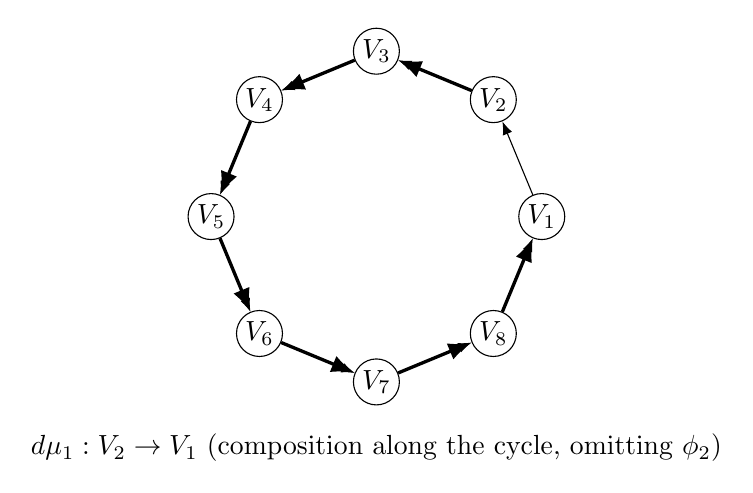
\begin{tikzpicture}[scale=1.05, every node/.style={circle,draw,inner sep=1.2pt}, >=Latex]
        % vertices on a circle
        \def\R{2.0}
        \foreach \i in {1,...,8} {
            \node (v\i) at ({\R*cos(360*(\i-1)/8)},{\R*sin(360*(\i-1)/8)}) {$V_{\i}$};
        }
        % cycle arrows
        \foreach \i [evaluate=\i as \j using {int(mod(\i,8)+1)}] in {1,...,8} {
            \draw[->] (v\i) -- (v\j);
        }
        % highlight a representative path for d\mu_l
        \draw[->,very thick] (v2) -- (v3);
        \draw[->,very thick] (v3) -- (v4);
        \draw[->,very thick] (v4) -- (v5);
        \draw[->,very thick] (v5) -- (v6);
        \draw[->,very thick] (v6) -- (v7);
        \draw[->,very thick] (v7) -- (v8);
        \draw[->,very thick] (v8) -- (v1);
        \node[draw=none,rectangle] at (0,-2.8) {$d\mu_{1}: V_2\to V_1$ (composition along the cycle, omitting $\phi_2$)};
    \end{tikzpicture}
    \caption{The cyclic quiver $C_n$ (illustrated here with $n=8$). The thick arrows indicate the path whose composition gives a typical $d\mu_l$ map along the cycle (example: $d\mu_{2}:V_2\to V_1$).}
\end{figure}

\begin{proposition}[Equivariance of the cyclic composition maps]\label{prop:mu-equivariant}
Let $C_{L+1}$ be the cyclic quiver on vertices $\{0,\ldots,L\}$, let $\mathrm{Rep}_{d}(C_{L+1})$ be its representation space with
$V_l\cong\mathbb{R}^{d_l-r}$, and let
\[\phi=(\phi_1,\ldots,\phi_L,\phi_{L+1})\in \Rep_d(C_{L+1}).\]
Define the base--change group
\[
G_d:=\prod_{l=0}^{L} \mathrm{GL}(V_l)
\]
acting on $\mathrm{Rep}_{d}(C_{L+1})$ via
\[
(g\cdot \phi)_l := g_l\,\phi_l\,g_{l-1}^{-1},\quad (l=0,\ldots,L), \ \text{mod} \ L+1
\]
For each $l=1,\ldots,L$, define
\[
d\mu_l(\phi) := \phi_{l-1}\cdots\phi_1\,\phi_{L+1}\,\phi_L\cdots\phi_{l+1}\in\mathrm{Hom}(V_{l+1},V_l),
\]
with the convention that an empty product is the identity.
Then, for all $g\in G_d$ and all $l=0,\ldots,L$,
\[
d\mu_l(g\cdot \phi) = g_l\,d\mu_l(\phi)\,g_{l+1}^{-1}.
\]
\end{proposition}

\begin{proof}
Expand $d\mu_l(g\cdot\phi)$ as a product of the maps $(g\cdot\phi)_i$. Each factor contributes a left multiplication by some $g_i$ and a right multiplication by $g_{i+1}^{-1}$, and all intermediate terms cancel by associativity, leaving only $g_l$ on the left and $g_{l+1}^{-1}$ on the right.
\end{proof}

\begin{proposition}[Orbit decomposition of $\Gamma_d$]\label{prop:GammaC-orbits}
Let
\[
\Gamma_d:=\Big\{\phi\in \mathrm{Rep}_{d}(C_{L+1})\ \Big|\ d\mu_l(\phi)=0\ \text{for all }l=1,\ldots,L\Big\}.
\]
Then $\Gamma_d$ is $G_d$-invariant. In particular, $\Gamma_d$ decomposes as a disjoint union of $G_d$-orbits:
\[
\Gamma_d = \bigsqcup_{\phi\in \Gamma_d} G_d\cdot \phi.
\]
\end{proposition}

\begin{proof}
By Proposition~\ref{prop:mu-equivariant}, each map $d\mu_l$ is $G_d$-equivariant and hence the vanishing set $d\mu_l^{-1}(0)$ is $G_d$-stable. Intersecting over $l=1,\ldots,L$ shows that $\Gamma_d$ is $G_d$-stable. Any group action partitions a set into disjoint orbits, yielding the stated decomposition.
\end{proof}
Note that $\Gamma_d\cong \Rep_d(C_{L+1})/< d\mu_l > $ is then finite dimensional and we can clasified indecomposable using indecomposable representations of Nakayama algebras.
\subsection{Cyclic quiver as a bounded module}
\begin{definition}[Path algebra]
Let $Q$ be a quiver. The \emph{path algebra} $kQ$ is the $k$-vector space with basis given by all directed paths in $Q$ (including the trivial paths $e_i$ of length $0$ at each vertex $i$), with multiplication given by concatenation of composable paths and $0$ otherwise, extended by bilinearity.
\end{definition}

\begin{definition}[Bound quiver algebra associated with $\Gamma_d$]
Let $Q=C_{L+1}$ and for each $l=0,\ldots,L$ let $p_l\in kQ$ be the path
\[
 p_l := a_{l-1}\cdots a_1\,a_{L+1}\cdots a_{l+1},
\]
interpreting empty products as the corresponding trivial path.
Let $I\subset kQ$ be the two-sided ideal generated by $\{p_1,\ldots,p_{L}\}$.
The quotient algebra
\[
A:=kQ/I
\]
is called the \emph{bound quiver algebra} associated with these relations.
\end{definition}

\begin{definition}[Representation of an algebra of dimension $d$]
Let $A$ be a $k$-algebra and let $d=(d_0,\ldots,d_L)$.
A \emph{representation of $A$ of dimension $d$ compatible with the vertices} is a left $A$-module structure on
$V:=\bigoplus_{i=0}^L k^{d_i}$ such that the idempotents $e_i\in kQ\twoheadrightarrow A$ act as the projections onto the $i$-th summand.
We denote the corresponding representation space by $\mathrm{Rep}_d(A)$.
\end{definition}

\begin{proposition}[From quiver representations with relations to $A$-modules]
There is a well-defined map
\[
F:\Gamma_d\to \mathrm{Rep}_d(A)
\]
which sends $\phi\in\Gamma_d$ to the unique $A$-module structure on $V$ for which each arrow $a_i$ acts by the linear map $\phi_i$.
\end{proposition}

\begin{proof}
Given $\phi\in\Gamma_d$, the tuple of linear maps $(\phi_i)_i$ defines a representation of the quiver $Q=C_{L+1}^{op}$, hence a left $kQ$-module structure on $V$ by letting a path act by the corresponding composition of arrow maps.
For each $l$, the defining condition $\mu_l(\phi)=0$ is exactly the statement that the element $p_l\in kQ$ acts as the zero map on $V$.
Since $I$ is the two-sided ideal generated by the $p_l$, every element of $I$ also acts by zero.
Therefore the $kQ$-action factors through the quotient $A=kQ/I$, producing a unique $A$-module structure on $V$ with the required arrow actions.
\end{proof}

\begin{proposition}[From $A$-modules to quiver representations with relations]
There is a well-defined map
\[
G:\mathrm{Rep}_d(A)\to \Gamma_d
\]
which sends an $A$-module structure on $V$ to the induced quiver representation $\phi$ whose arrow maps are the actions of the classes of the arrows $a_i$.
\end{proposition}

\begin{proof}
Let $V$ be a representation in $\mathrm{Rep}_d(A)$.
Composing the action map $A\to \mathrm{End}_k(V)$ with the quotient map $kQ\twoheadrightarrow A$ gives a $kQ$-module structure on $V$.
Restricting the action of each arrow basis element $a_i$ to the appropriate vertex summand yields linear maps $\phi_i:V_i\to V_{i+1}$ and hence a point $\phi\in\mathrm{Rep}_d(C_n)$.
Because each $p_l$ maps to zero in $A$, it acts as the zero endomorphism on $V$.
Equivalently, the composed linear map $\mu_l(\phi)$ is zero for every $l$, so $\phi\in\Gamma_d$.
\end{proof}

\begin{proposition}[Correspondence between $\Gamma_d$ and $\mathrm{Rep}_d(A)$]
The maps $F$ and $G$ are mutually inverse bijections. In particular,
\[
\Gamma_d \cong \mathrm{Rep}_d(A),\qquad A=kQ/I.
\]
\end{proposition}

\begin{proof}
Starting from $\phi\in\Gamma_d$, the $A$-module $F(\phi)$ is by construction generated by the same arrow actions as $\phi$, so applying $G$ recovers the same tuple of arrow maps, hence $G(F(\phi))=\phi$.
Conversely, starting from an $A$-module structure on $V$, the map $G$ records the arrow actions and the map $F$ reconstructs the unique $A$-module whose arrow actions agree with those recorded, hence $F(G(V))=V$.
\end{proof}
\begin{lemma}[Finite-dimensionality of $A=kQ/I$]\label{lem:A-finite-dim}
Let $Q=C_{L+1}$ be the oriented cycle on $L+1$ vertices, and let $I\subset kQ$ be the two-sided ideal generated by the paths
$p_1,\dots,p_{L}$, where each $p_l$ is a path of length $L$ (the unique directed path going around the cycle while omitting one arrow).
Then every directed path in $Q$ of length $\ge L +1$ lies in $I$. In particular, $A=kQ/I$ is finite-dimensional.
\end{lemma}

\begin{proof}
Let $q$ be any directed path in $Q$ of length $\ge L+1$. Write $q=b_m b_{m-1}\cdots b_1$ as a concatenation of arrows with $m\ge L+1$.
Consider the contiguous subpath $q':=b_{L}\cdots b_1$ of length $L$. Since $Q$ is an oriented $L+1$-cycle, there is exactly one directed
path of length $L$ from its source to its target, hence $q'$ must coincide with one of the generators $p_l$.
Therefore $q=q''\,p_l$ for some (possibly trivial) path $q''$, so $q\in I$ because $I$ is a two-sided ideal.

Thus all paths of length $\ge L+1$ vanish in $A$, so $A$ is spanned by the residue classes of paths of length $<L+1$, a finite set. Hence $A$ is finite-dimensional.
\end{proof}

\subsection{Bounded modules are Nakayama algebras}
\begin{definition}[$A$-module]
Let $A$ be a (not necessarily commutative) $k$-algebra.
A (left) \emph{$A$-module} is a $k$-vector space $M$ together with a $k$-bilinear map
\[
A\times M\to M,\qquad (a,m)\mapsto a\cdot m,
\]
such that for all $a,b\in A$ and $m\in M$ one has
\[
(ab)\cdot m = a\cdot (b\cdot m),\qquad 1_A\cdot m = m.
\]
A \emph{homomorphism} of $A$-modules is a $k$-linear map commuting with the $A$-action.
\end{definition}

\begin{definition}[Indecomposable module]
An $A$-module $M$ is \emph{indecomposable} if $M\neq 0$ and there do not exist nonzero submodules $M_1,M_2\subset M$ such that
\[
M \cong M_1\oplus M_2.
\]
Equivalently, $M$ is indecomposable if every idempotent endomorphism of $M$ is either $0$ or $\mathrm{id}_M$.
\end{definition}

\begin{definition}[Composition series]
Let $M$ be a finite-dimensional $A$-module.
A \emph{composition series} of $M$ is a finite chain of submodules
\[
0=M_0\subset M_1\subset \cdots \subset M_{\ell}=M
\]
such that each successive quotient $M_i/M_{i-1}$ is \emph{simple}.
The integer $\ell$ is called the \emph{length} of the series.
\end{definition}

\begin{definition}[Projective module]
An $A$-module $P$ is \emph{projective} if for every surjective $A$-module homomorphism $f:M\twoheadrightarrow N$ and every $A$-module homomorphism $g:P\to N$, there exists an $A$-module homomorphism $\tilde g:P\to M$ such that $f\circ \tilde g=g$.
Equivalently, $P$ is projective if the functor $\mathrm{Hom}_A(P,-)$ is exact.
\end{definition}

\begin{definition}[Indecomposable projective module]
A \emph{projective indecomposable} $A$-module is an $A$-module that is both projective and indecomposable.
For a finite-dimensional basic algebra $A$, every indecomposable projective module is of the form $P_i\cong Ae_i$ for a primitive idempotent $e_i\in A$, and every projective module decomposes uniquely as a direct sum of indecomposable projectives.
\end{definition}

\begin{definition}[Uniserial module]
An $A$-module $M$ is \emph{uniserial} if it admits a unique composition series. Equivalently, the set of submodules of $M$ is totally ordered by inclusion.
\end{definition}
\begin{definition}[\textbf{Nakayama algebra}]
Let $A$ be a finite-dimensional $k$-algebra. We say that $A$ is a \emph{Nakayama algebra} if every indecomposable left $A$-module is \emph{uniserial}, i.e.\ it admits a unique composition series.
Equivalently, $A$ is Nakayama if every indecomposable projective left $A$-module is uniserial (and hence every indecomposable injective is uniserial).
\end{definition}

\begin{definition}[Admissible ideal]
Let $Q$ be a finite quiver and let $kQ$ be its path algebra. Write $(kQ)_{\ge m}$ for the $k$-span of all paths of length at least $m$.
A two-sided ideal $I\subset kQ$ is called \emph{admissible} if there exists an integer $m\ge 2$ such that
\[
(kQ)_{\ge m}\subseteq I \subseteq (kQ)_{\ge 2}.
\]
\end{definition}

\begin{definition}[Jacobson radical]
Let $A$ be a (not necessarily commutative) ring. The \emph{Jacobson radical} $J(A)$ is the intersection of all maximal left ideals of $A$.
If $A$ is a finite-dimensional $k$-algebra, then equivalently
\[
J(A)=\bigcap_{S\ \text{simple}} \ker\big(A\to \mathrm{End}_k(S)\big),
\]
i.e.\ $J(A)$ is the largest two-sided ideal that acts by zero on every simple $A$-module.
\end{definition}

\begin{proposition}[\textbf{Bound quiver criterion for Nakayama algebras}]\label{prop:bound-quiver-nakayama}
Let $A \simeq kQ/I$ be a finite-dimensional bound quiver algebra, where $Q$ is a finite quiver and
$I\subset kQ$ is an admissible ideal.
Assume that for every vertex $i\in Q_0$ there is at most one arrow leaving $i$ and at most one arrow entering $i$.
Then $A$ is a Nakayama algebra.

Moreover, if $Q$ is connected and has exactly one arrow leaving and exactly one arrow entering each vertex, then $Q$ is an oriented cycle and $A$ is a \emph{cyclic Nakayama algebra}. If instead $Q$ is connected and has a unique source and a unique sink, then $Q$ is an oriented line and $A$ is a \emph{linear Nakayama algebra}.
\end{proposition}

\begin{proof}
Let $e_i\in kQ\twoheadrightarrow A$ be the primitive idempotent corresponding to a vertex $i\in Q_0$, and consider the indecomposable projective module $P_i := Ae_i$.
As a $k$-vector space, $P_i$ is spanned by residue classes of paths in $Q$ starting at $i$ (modulo the relations in $I$).
Because there is at most one arrow leaving each vertex, for each $\ell\ge 0$ there is \emph{at most one} directed path of length $\ell$ starting at $i$; hence $P_i$ has a basis indexed by (the surviving classes of) these paths.

Let $J\subset A$ denote the Jacobson radical. Since $A\simeq kQ/I$ with $I$ admissible, $J$ is generated (as a two-sided ideal) by the classes of arrows, and one has
\[
J^\ell P_i = J^\ell Ae_i \ \cong\ (J^\ell)e_i,
\]
which is spanned by classes of paths of length $\ge \ell$ starting at $i$.
By the previous paragraph, for each $\ell$ the quotient $J^\ell P_i/J^{\ell+1}P_i$ is either $0$ or a simple module (it is spanned by the class of the unique surviving path of length $\ell$, if it exists).
Therefore the radical filtration
\[
P_i \supset JP_i \supset J^2P_i \supset \cdots
\]
is a chain whose successive quotients are simple (or zero), i.e.\ $P_i$ is uniserial.

Thus every indecomposable projective $P_i$ is uniserial, and hence $A$ is a Nakayama algebra.

For the final statements: if $Q$ is connected and every vertex has exactly one incoming and one outgoing arrow, then the underlying directed graph is a directed cycle. If $Q$ is connected and has a unique source and sink with all other vertices having one incoming and one outgoing arrow, then the directed graph is a directed line. These correspond to cyclic and linear Nakayama algebras respectively.
\end{proof}
\subsection{Cyclic monomial Nakayama algebra with uniform Kupisch series}
Throughout this subsection, let $Q=C_{L+1}$ be the oriented $L+1$-cycle, let $kQ$ be its path algebra, and let
\[
A:=kQ/I
\]
be the bound quiver algebra from Definition~(Bound quiver algebra associated with $\Gamma_d$).

\begin{definition}[Monomial (path) ideal / monomial algebra]
An ideal $I\subset kQ$ is called \emph{monomial} if it is generated (as a two-sided ideal) by paths in $Q$.
A quotient $kQ/I$ with $I$ monomial is called a \emph{monomial algebra}.
\end{definition}

\begin{definition}[Kupisch series]
Let $A$ be a finite-dimensional basic algebra with primitive idempotents $e_1,\ldots,e_{L+1}$ and indecomposable projectives
$P_i:=Ae_i$.
The \emph{Kupisch series} of $A$ is the $L+1$-tuple
\[
(c_1,\ldots,c_{L+1}),\qquad c_i:=\ell(P_i),
\]
where $\ell(P_i)$ denotes the composition length of $P_i$.
\end{definition}

\begin{remark}[Loewy length]
For a finite-dimensional algebra $A$ with Jacobson radical $J=J(A)$, the \emph{Loewy length} is the smallest integer $n$ such that $J^n=0$.
\end{remark}

\begin{proposition}[Identification and Kupisch series]
With $Q=C_{L+1}$ and $I=(p_1,\ldots,p_{L+1})$ as above, the algebra $A=kQ/I$ is a \emph{cyclic monomial Nakayama algebra}.
Moreover its Kupisch series is uniform:
\[
(c_1,\ldots,c_{L+1})=(L,\ldots,L).
\]
\end{proposition}

\begin{proof}
By construction, the ideal $I$ is generated by the paths $p_1,\ldots,p_{L+1}$, hence $I$ is monomial and $A$ is a monomial algebra.
By Proposition~\ref{prop:bound-quiver-nakayama}, $A$ is Nakayama; since $Q=C_{L+1}$ is an oriented cycle, $A$ is in fact \emph{cyclic} Nakayama.

Fix a vertex $i$ and consider $P_i=Ae_i$.
Modulo $I$, every path in $Q$ of length $\ge L$ starting at $i$ vanishes, while for each $t=0,1,\ldots,L-1$ there is exactly one directed path of length $t$ starting at $i$.
Therefore $P_i$ has a $k$-basis given by the residue classes of these $L$ paths (length $0$ through $L-1$).

Since $J=J(A)$ is generated by the classes of arrows (as recalled in the proof of Proposition~\ref{prop:bound-quiver-nakayama}), the radical filtration
\[
P_i \supset JP_i \supset J^2P_i \supset \cdots
\]
has successive quotients $J^tP_i/J^{t+1}P_i$ one-dimensional (hence simple) for $t=0,\ldots,L-1$, and zero thereafter.
Thus $\ell(P_i)=L$ for every $i$, which gives the Kupisch series $(L,\ldots,L)$.
\end{proof}

\begin{remark}
Equivalently, $A$ can be viewed as a \emph{truncated cycle algebra}: it is the path algebra of an oriented cycle with all paths of length $\ge L$ killed.
\end{remark}
\subsection{Indecomposable representations of Nakayama algebras}
\begin{definition}[The uniserial modules $M(i,\ell)$]
Fix $Q=C_{L+1}$ with vertices $Q_0=\{0,\dots,L\}$ and arrows $a_i:l-1\to l$ for $l=1,\dots,L$ and $a_{L+1}:L\to 0$.
For $i\in Q_0$ and $0\le \ell\le L$, define a representation $M(i,\ell)$ of $Q$ by
\[
M(i,\ell)_j :=
\begin{cases}
k, & j\in\{i,i+1,\dots,i+\ell-1\}\ (\mathrm{mod}\ L + 1),\\
0, & \text{otherwise},
\end{cases}
\]
and for each arrow $a_j:j-1\to j$,
\[
M(i,\ell)_{a_j} :=
\begin{cases}
\mathrm{id}_k, & \text{if both source and target are }k,\\
0, & \text{otherwise}.
\end{cases}
\]
\end{definition}

\begin{lemma}[The relations vanish on $M(i,\ell)$]\label{lem:Miell-well-defined}
Let $Q=C_{L+1}$ and, for each $l\in\{1,\dots,L+1\}$, let
\[
p_l := a_{l-1}\cdots a_1\, a_{L+1}\cdots a_{l+1}
\]
be the oriented path of length $L$ going once around the cycle and omitting $a_l$.
Set $A:=kQ/\langle p_1,\dots,p_{L+1}\rangle$.
Then, for every $i\in Q_0$ and $1\le \ell\le L$, the representation $M(i,\ell)$ factors through $A$, hence defines a finite-dimensional left $A$-module.
\end{lemma}

\begin{proof}
Fix $i$ and $\ell$. Each path $p_l$ has length $L$.
Since the support of $M(i,\ell)$ contains only $\ell\le L$ consecutive vertices, the corresponding composition along $p_l$ necessarily passes through a vertex where $M(i,\ell)$ is zero.
Therefore $p_l$ acts by the zero map on $M(i,\ell)$ for every $l$, so all generators of the ideal $\langle p_1,\dots,p_{L}\rangle$ act trivially.
Hence the $kQ$-action factors through $A$.
\end{proof}

\begin{lemma}[Uniseriality of $M(i,\ell)$]\label{lem:Miell-uniserial}
For every $i\in Q_0$ and $1\le \ell\le L + 1$, the $A$-module $M(i,\ell)$ is uniserial, and in particular indecomposable.
\end{lemma}

\begin{proof}
Any nonzero submodule $N\subseteq M(i,\ell)$ must contain the one-dimensional space at some vertex in the support.
Because all arrow maps inside the support are identities, containing a vertex forces $N$ to contain all vertices reachable along the directed arrows within the support.
Consequently, the nonzero submodules are exactly the modules
$M(i+t,\ell-t)$ for $t=0,\dots,\ell-1$ (indices taken modulo $n$), and they form a chain under inclusion.
Thus submodules are totally ordered and $M(i,\ell)$ is uniserial.
\end{proof}

\begin{lemma}[Endomorphisms of $M(i,\ell)$]\label{lem:Miell-end}
For every $i\in Q_0$ and $1\le \ell\le L$, one has $\mathrm{End}_A\big(M(i,\ell)\big)\cong k$.
\end{lemma}

\begin{proof}
Let $f\in \mathrm{End}_A(M(i,\ell))$.
On each vertex $j$ in the support, $f$ is multiplication by some scalar $\lambda_j\in k$.
For each arrow inside the support, the arrow map is $\mathrm{id}_k$, so commutativity forces $\lambda_{j+1}=\lambda_j$.
Hence all $\lambda_j$ coincide with a single scalar $\lambda$, and $f=\lambda\,\mathrm{id}$.
\end{proof}

\begin{lemma}[Projective truncations realize $M(i,\ell)$]\label{lem:Miell-as-truncation}
Let $P(i):=Ae_i$ be the indecomposable projective at vertex $i$ and let $J:=J(A)$.
Then, for every $i\in Q_0$ and $1\le \ell\le L$, there is an isomorphism of $A$-modules
\[
P(i)/J^{\ell}P(i)\ \cong\ M(i,\ell).
\]
\end{lemma}

\begin{proof}
By Proposition~\ref{prop:bound-quiver-nakayama} and the previous subsection, $A$ is a cyclic Nakayama algebra with uniform Kupisch series $(L,\ldots,L)$.
In particular, $P(i)$ is uniserial of length $L$, and $J^tP(i)$ is spanned by residue classes of paths of length $\ge t$ starting at $i$.
Thus $P(i)/J^{\ell}P(i)$ has a basis given by the residue classes of the unique paths of lengths $0,1,\dots,\ell-1$ starting at $i$.
Under the induced quiver description, this quotient has one-dimensional spaces on the vertices $i,i+1,\dots,i+\ell-1$ (mod $L+1$) and identity maps along arrows inside the support, which is exactly $M(i,\ell)$.
\end{proof}

\begin{proposition}[Indecomposable representations of the cyclic truncated Nakayama algebra]
\label{prop:indecomp-cyclic-nakayama}
Let $Q=C_{L+1}$ be the oriented cyclic quiver with arrows $a_i:i\to i+1$ for $i=1,\dots,L$ and $a_{L+1}:L\to 0$.
For each $l\in\{1,\dots,L+1\}$, let $p_l$ be the path of length $L$ going once around the cycle and omitting $a_l$, and set
\[
A := kQ / \langle p_1,\dots,p_{L+1}\rangle.
\]
Then every finite-dimensional indecomposable left $A$-module is isomorphic to a unique module $M(i,\ell)$ with $i\in Q_0$ and $1\le \ell\le L$.
Equivalently, every indecomposable $A$-module is of the form $P(i)/J^{\ell}P(i)$ for a unique pair $(i,\ell)$.
In particular, $A$ has exactly $(L+1)L$ indecomposable modules up to isomorphism.
\end{proposition}

\begin{proof}
By Lemma~\ref{lem:Miell-well-defined}, each $M(i,\ell)$ is a well-defined finite-dimensional $A$-module, and by Lemma~\ref{lem:Miell-uniserial} it is indecomposable.

Conversely, since $A$ is Nakayama (Proposition~\ref{prop:bound-quiver-nakayama}), every indecomposable $A$-module is uniserial and hence a quotient of a unique indecomposable projective $P(i)=Ae_i$.
Its composition length is some $\ell$ with $1\le \ell\le \ell(P(i))=L$, and uniseriality forces the quotient to be $P(i)/J^{\ell}P(i)$.
By Lemma~\ref{lem:Miell-as-truncation}, this module is isomorphic to $M(i,\ell)$.

Uniqueness follows because the top simple module determines $i$ and the length determines $\ell$.
Counting pairs $(i,\ell)$ with $i\in Q_0$ and $1\le \ell\le L$ gives $(L+1)L$.
\end{proof}
More details about this can be found in the following lecture notes:
\href{https://www.math.uni-bielefeld.de/~wcrawley/1920noncommalg2/NA2.pdf}{Noncommutative Algebra 2: Representations of finite-dimensional algebras} in particular theorem and corroloray section 1.6.
We have a Krull schmidt theorem for these Nakayama algebras.
\begin{proposition}[Krull--Schmidt for the cyclic truncated Nakayama algebra]\label{prop:KS-cyclic-truncated-nakayama}
Let $A=kQ/I$ be the cyclic truncated Nakayama algebra, where $Q=C_{L+1}$ is the oriented $L+1$-cycle and $I$ is the ideal generated by the length-$(L)$ paths $p_1,\dots,p_{L+1}$ (equivalently, all paths of length $\ge L+1$ vanish in $A$).
Let $\mathrm{mod}\text{-}A$ denote the category of finite-dimensional left $A$-modules.
Then every $M\in \mathrm{mod}\text{-}A$ admits a decomposition as a finite direct sum of indecomposable $A$-modules.
Moreover, this decomposition is unique up to reordering and isomorphism of the indecomposable summands.
Equivalently, using the explicit indecomposables $M(i,\ell)$ from Proposition~\ref{prop:indecomp-cyclic-nakayama}, there exist uniquely determined multiplicities
$m_{i,\ell}\in\mathbb{Z}_{\ge 0}$ such that
\[
M \ \cong\ \bigoplus_{i=0}^{L} \ \bigoplus_{\ell=1}^{L} \ M(i,\ell)^{\oplus m_{i,\ell}}.
\]
\end{proposition}

\begin{proof}[Proof sketch]
Since $A$ is finite-dimensional over $k$, it is left artinian (and left noetherian), hence every object of $\mathrm{mod}\text{-}A$ has finite length.
In particular, $\mathrm{mod}\text{-}A$ is a Krull--Schmidt category: every object decomposes as a finite direct sum of indecomposables, and such a decomposition is unique up to permutation and isomorphism.

Concretely, existence follows by choosing a nonzero module $M$ and repeatedly splitting off a nontrivial direct summand until all summands are indecomposable; the process terminates because $M$ has finite length.
Uniqueness follows because each indecomposable has a local endomorphism ring (for example, by Lemma~\ref{lem:Miell-end} in the explicit classification), and the classical Krull--Schmidt--Azumaya argument applies.

Finally, Proposition~\ref{prop:indecomp-cyclic-nakayama} classifies the indecomposables as the modules $M(i,\ell)$, so any Krull--Schmidt decomposition can be rewritten uniquely in the stated multiplicity form.
\end{proof}
\textbf{Note}: This enables to parameterize the orbits of $\Gamma$ with the indecomposables representations.
\paragraph{Orbits, isomorphism classes, and multiplicity patterns.}
Fix a finite-dimensional $k$-algebra $A$ and a dimension vector $d=(d_0,\dots,d_{L})$.
Recall that
\[
\mathrm{Rep}_d(A)
=\Big\{\text{left $A$-module structures on }V=\bigoplus_{i=0}^{L} k^{d_i}\text{ such that each idempotent $e_i$ acts as the projection onto }k^{d_i}\Big\}.
\]
Let
\[
G_d:=\prod_{i=0}^{L} \mathrm{GL}(k^{d_i})
\]
act on $\mathrm{Rep}_d(A)$ by \emph{change of bases at the vertices} (equivalently, by transport of structure):
for $g=(g_0,\dots,g_L)\in G_d$ and a module structure $\rho:A\to \mathrm{End}_k(V)$, define a new module
structure $g\cdot \rho$ by
\[
(g\cdot \rho)(a)\;:=\; g\,\rho(a)\,g^{-1},\qquad g:=\bigoplus_{i=1}^n g_i\in \mathrm{GL}(V).
\]
When $A\simeq kQ/I$ is presented as a bound quiver algebra, this action is equivalently given on arrow
maps by $(g\cdot \phi)_a=g_{t(a)}\,\phi_a\,g_{s(a)}^{-1}$.
Then two points $\rho,\rho'\in \mathrm{Rep}_d(A)$ lie in the same $G_d$-orbit if and only if the corresponding
$A$-modules $(V,\rho)$ and $(V,\rho')$ are isomorphic in $\mathrm{mod}\text{-}A$.
Consequently, there is a canonical bijection
\[
\big(G_d\backslash \mathrm{Rep}_d(A)\big)\ \cong\ \Big\{\text{isomorphism classes of $A$-modules $M$ with $\dim(e_iM)=d_i$ for all $i$}\Big\}.
\]

Now specialize to the cyclic truncated Nakayama algebra $A=kQ/I$ considered above.
Its indecomposable modules are the uniserials $M(i,\ell)$ with $i\in\{0,\dots,L\}$ (indices taken modulo $L+1$) and $1\le \ell\le L$
(Proposition~\ref{prop:indecomp-cyclic-nakayama}).
By the Krull--Schmidt theorem (Proposition~\ref{prop:KS-cyclic-truncated-nakayama}), every finite-dimensional
$A$-module $M$ admits a decomposition
\[
M\ \simeq\ \bigoplus_{i=0}^{L}\ \bigoplus_{\ell=1}^{L} M(i,\ell)^{\oplus m_{i,\ell}},
\qquad m_{i,\ell}\in\mathbb{Z}_{\ge 0},
\]
and this decomposition is unique up to permutation of summands.
The multiplicities $(m_{i,\ell})$ determine (and are constrained by) the dimension vector $d$ via the \emph{covering equations}
\begin{equation}\label{eq:cyclic-multiplicity-constraints}
d_k \;=\; \sum_{i=0}^{L}\ \sum_{\ell=1}^{L} m_{i,\ell}\,\mathbf{1}\!\left\{k\in\{i,i+1,\dots,i+\ell-1\}\ (\mathrm{mod}\ L+1)\right\},
\qquad k=0,\dots,L,
\end{equation}
since $M(i,\ell)$ contributes a one-dimensional space at vertex $k$ exactly when $k$ lies in its cyclic
support interval of length $\ell$ starting at $i$.
Define the set of \emph{multiplicity patterns}
\[
M_d^{+}(A)
:=\left\{(m_{i,\ell})\in \mathbb{Z}_{\ge 0}^{L(L+1)}\ \middle|\ \text{\eqref{eq:cyclic-multiplicity-constraints} holds for all }k\right\}.
\]
Then the above discussion yields a concrete parametrization of orbits:
every $G_d$-orbit in $\mathrm{Rep}_d(A)$ corresponds to a unique isomorphism class in $\mathrm{mod}\text{-}A$,
and hence to a unique multiplicity pattern $(m_{i,\ell})\in M_d^{+}(A)$ via its Krull--Schmidt decomposition.
In other words, we obtain canonical bijections
\[
G_d\backslash \mathrm{Rep}_d(A)
\ \cong\
\Big\{\text{isomorphism classes in $\mathrm{mod}\text{-}A$ with dimension vector $d$}\Big\}
\ \cong\
M_d^{+}(A),
\]
where the last map sends an $A$-module to the multiplicities of the indecomposables $M(i,\ell)$ in its Krull--Schmidt decomposition.
\begin{proposition}[Orbit stratification of $\Gamma_d$ by indecomposable Nakayama modules]
\label{prop:Gamma_orbit_stratification}

Fix $L \ge 1$ and let $Q = C_{L+1}$ be the oriented cyclic quiver on vertices
$\{0,\dots,L\}$.  
Let $A := kQ/I$ be the bound quiver algebra, where $I$ is the ideal generated by the length-$L$
paths $p_1,\dots,p_{L+1}$ obtained by going once around the cycle and omitting one arrow.
Let $d=(d_0,\dots,d_L)$ be a dimension vector.

Define
\[
\Gamma_d := \left\{
\phi \in \mathrm{Rep}_d(Q)
\;\middle|\;
d\mu_\ell(\phi)=0 \text{ for all } \ell=1,\dots,L
\right\},
\]
where
\[
d\mu_\ell(\phi) := \phi_{\ell-1}\cdots \phi_1\,\phi_{L+1}\,\phi_L\cdots \phi_{\ell+1}.
\]

Let
\[
G_d := \prod_{i=0}^{L} \mathrm{GL}(k^{d_i})
\]
act on $\Gamma_d$ by base change at the vertices.

\medskip

Then the following hold.

\begin{enumerate}
\item
There is a canonical identification
\[
\Gamma_d \;\cong\; \mathrm{Rep}_d(A),
\]
under which the $G_d$-action coincides with transport of structure on $A$-modules.

\item
The algebra $A$ is a finite-dimensional cyclic Nakayama algebra.  
Its indecomposable finite-dimensional left modules are, up to isomorphism, the uniserial modules
\[
M(i,\ell), \qquad i \in \{0,\dots,L\}, \quad 1 \le \ell \le L,
\]
supported on $\ell$ consecutive vertices starting at $i$ (indices taken modulo $L+1$).

\item
Every $A$-module $M$ of dimension vector $d$ admits a unique (up to permutation)
Krull--Schmidt decomposition
\[
M \;\cong\; \bigoplus_{i=0}^{L}\;\bigoplus_{\ell=1}^{L} M(i,\ell)^{\oplus m_{i,\ell}},
\]
for uniquely determined multiplicities $m_{i,\ell} \in \mathbb{Z}_{\ge 0}$ satisfying the
dimension constraints
\[
d_k \;=\;
\sum_{i=0}^{L}\sum_{\ell=1}^{L}
m_{i,\ell}\,
\mathbf{1}\!\left\{
k \in \{i,i+1,\dots,i+\ell-1\} \ (\mathrm{mod}\ L+1)
\right\},
\quad k=0,\dots,L.
\]

Denote by $\mathcal M_d^+(A)$ the finite set of all such multiplicity patterns
$m=(m_{i,\ell})$.

\item
For each $m \in \mathcal M_d^+(A)$, define the stratum
\[
\Gamma_d^{(m)}
:=
\left\{
\phi \in \Gamma_d
\;\middle|\;
F(\phi) \cong
\bigoplus_{i,\ell} M(i,\ell)^{\oplus m_{i,\ell}}
\right\},
\]
where $F(\phi)$ denotes the associated $A$-module.

Then $\Gamma_d^{(m)}$ is a single $G_d$-orbit.

\item
The variety $\Gamma_d$ decomposes as a disjoint union of these orbits:
\[
\Gamma_d
\;=\;
\bigsqcup_{m \in \mathcal M_d^+(A)} \Gamma_d^{(m)}
\;=\;
\bigsqcup_{m \in \mathcal M_d^+(A)} G_d \cdot \phi_m,
\]
where $\phi_m$ is any representative whose associated $A$-module has multiplicity pattern $m$.
\end{enumerate}

\noindent
In particular, the $G_d$-orbits in $\Gamma_d$ are canonically parameterized by the
multiplicity data of indecomposable $A$-modules, i.e.\ by the set
$\mathcal M_d^+(A)$.
\end{proposition}



\section{Stratification of $\Gamma_{XY}$}
While the indecomposable representation of $\Gamma$ are parameterized by the $M(i,\ell)$ from the previous modules over Nakayama algebras we are actually interested in decomposing:
\begin{equation*}
    \Gamma_{\sigma} := \left\{(\phi_1,\ldots,\phi_{L+1})\in \mathrm{Rep}_d(C_{L+1})\;\middle|\; \phi_{l-1}\cdots\phi_1\,\phi_{L+1}\,\phi_L\cdots\phi_{l+1} = 0,\; \phi_{L+1}=\sigma\right\}.
\end{equation*}
where the map $\sigma\in \mathrm{Hom}(V_L,V_0)$ is fixed (in DLN it is $\Sigma_{XY}U_Q$).
The map
\begin{equation*}
    d\mu_{l,\sigma} := \phi_{l-1}\cdots\phi_1\,\sigma\,\phi_L\cdots\phi_{l+1}
\end{equation*}
is no longer $G_d$-equivariant.

\begin{definition}[Stabilizer group of the fixed arrow]\label{def:stabilizer-sigma}
Let $\sigma\in\mathrm{Hom}(V_L,V_1)$ be fixed. Define
\[
\mathrm{Stab}(\sigma):=\{(g_1,g_L)\in \mathrm{GL}(V_1)\times \mathrm{GL}(V_L)\mid g_1\,\sigma\,g_L^{-1}=\sigma\},
\]
and the corresponding subgroup of the base--change group
\[
G_\sigma:=\{g=(g_1,\ldots,g_L)\in \prod_{l=1}^L\mathrm{GL}(V_l)\mid (g_1,g_L)\in \mathrm{Stab}(\sigma)\}.
\]
\end{definition}

\begin{proposition}[$G_\sigma$-equivariance of the cyclic composition maps]\label{prop:mu-sigma-equivariant}
Fix $\sigma\in\mathrm{Hom}(V_L,V_1)$ and consider the representation space with $\phi_{L+1}=\sigma$.
For $\phi=(\phi_1,\ldots,\phi_L,\sigma)$ and each $l=1,\ldots,L$, define
\[
d\mu_{l,\sigma}(\phi):=\phi_{l-1}\cdots \phi_1\,\sigma\,\phi_L\cdots \phi_{l+1}\in\mathrm{Hom}(V_{l+1},V_l),
\]
with the convention that an empty product is the identity.
Then, for all $g\in G_\sigma$ and all $l$,
\[
d\mu_{l,\sigma}(g\cdot \phi)= g_l\,\mu_{l,\sigma}(\phi)\,g_{l+1}^{-1}.
\]
In particular, the subset $\Gamma_\sigma:=\bigcap_{l=1}^L d\mu_{l,\sigma}^{-1}(0)$ is $G_\sigma$-invariant.
\end{proposition}

\begin{proof}
Expand $d\mu_{l,\sigma}(g\cdot\phi)$ as a product of the maps $(g\cdot\phi)_i$.
All intermediate base-change factors cancel. The only remaining factors are $g_l$ on the left and
$g_{l+1}^{-1}$ on the right. The middle arrow is $(g\cdot\phi)_{L+1}=g_1\sigma g_L^{-1}$, which equals
$\sigma$ because $g\in G_\sigma$. 
\end{proof}
For all modules in $\Gamma_\sigma$ Krull-Schmidt applies (as a category of $A$-modules where $A$ is finite dimensional). We want to parameterize the orbits of $\Gamma_\sigma$ under the action of $G_\sigma$ and study their geometry (e.g. codimension).
\begin{lemma}[Intersection of a $G_d$--orbit with a fixed--arrow fiber]
\label{lem:orbit_fiber_intersection}
Let $L\ge 2$ and let $V_0,\dots,V_L$ be finite--dimensional vector spaces over an algebraically closed field $\Bbbk$.  
Set
\[
G_d \;:=\; \prod_{i=0}^L GL(V_i).
\]
Let $\Gamma_d$ be an affine variety equipped with an algebraic action of $G_d$.  
Assume there exists a morphism
\[
F:\Gamma_d \longrightarrow \Hom(V_L,V_0)
\]
satisfying the equivariance property
\begin{equation}
\label{eq:equivariance}
F(g\cdot x) \;=\; g_0\,F(x)\,g_L^{-1}
\qquad
\text{for all } g=(g_0,\dots,g_L)\in G_d,\; x\in\Gamma_d .
\end{equation}

Fix $\sigma\in \Hom(V_L,V_0)$ and define the fiber
\[
\Gamma_\sigma \;:=\; F^{-1}(\sigma).
\]
Define the stabilizer subgroup
\[
G_\sigma \;:=\; \{ g=(g_0,\dots,g_L)\in G_d \mid g_0\,\sigma\,g_L^{-1}=\sigma \}.
\]
Let $\mathcal O\subset \Gamma_d$ be a single $G_d$--orbit.  
Then either $\mathcal O\cap\Gamma_\sigma=\varnothing$, or else for every
$x\in\mathcal O\cap\Gamma_\sigma$ one has
\[
\mathcal O\cap\Gamma_\sigma \;=\; G_\sigma\cdot x .
\]
In particular, whenever $\mathcal O\cap\Gamma_\sigma\neq\varnothing$, this
intersection consists of a single $G_\sigma$--orbit.
\end{lemma}

\begin{proof}
We proceed in several steps.

\medskip\noindent
\textbf{Step 1: $\Gamma_\sigma$ is stable under the action of $G_\sigma$.}

Let $x\in\Gamma_\sigma$, so by definition $F(x)=\sigma$.  
Let $g\in G_\sigma$. Using the equivariance property \eqref{eq:equivariance},
\[
F(g\cdot x)
\;=\;
g_1\,F(x)\,g_L^{-1}
\;=\;
g_1\,\sigma\,g_L^{-1}.
\]
Since $g\in G_\sigma$, we have $g_1\,\sigma\,g_L^{-1}=\sigma$, and hence
$F(g\cdot x)=\sigma$. Therefore $g\cdot x\in\Gamma_\sigma$.  
This shows that $\Gamma_\sigma$ is invariant under the action of $G_\sigma$ and,
in particular,
\[
G_\sigma\cdot x \subseteq \Gamma_\sigma
\qquad
\text{for all } x\in\Gamma_\sigma .
\tag{$\ast$}
\]

\medskip\noindent
\textbf{Step 2: If $x\in\mathcal O\cap\Gamma_\sigma$, then
$G_\sigma\cdot x\subseteq \mathcal O\cap\Gamma_\sigma$.}

Let $x\in\mathcal O\cap\Gamma_\sigma$.  
Since $\mathcal O$ is a $G_d$--orbit, it is stable under the action of $G_d$ and
hence under the subgroup $G_\sigma\subseteq G_d$. Thus $G_\sigma\cdot x\subseteq
\mathcal O$.  
By $(\ast)$, $G_\sigma\cdot x\subseteq \Gamma_\sigma$.  
Combining these two inclusions gives
\[
G_\sigma\cdot x \subseteq \mathcal O\cap\Gamma_\sigma .
\tag{$\ast\ast$}
\]

\medskip\noindent
\textbf{Step 3: Any two points of $\mathcal O\cap\Gamma_\sigma$ differ by the
action of $G_\sigma$.}

Assume $x,y\in\mathcal O\cap\Gamma_\sigma$.  
Because $x$ and $y$ lie in the same $G_d$--orbit $\mathcal O$, there exists
$g=(g_1,\dots,g_L)\in G_d$ such that
\[
y = g\cdot x .
\]
Applying $F$ and using \eqref{eq:equivariance}, we obtain
\[
F(y)
\;=\;
F(g\cdot x)
\;=\;
g_1\,F(x)\,g_L^{-1}.
\]
Since $x,y\in\Gamma_\sigma$, we have $F(x)=F(y)=\sigma$. Therefore
\[
\sigma = g_1\,\sigma\,g_L^{-1}.
\]
By definition of $G_\sigma$, this implies $g\in G_\sigma$. Hence
$y=g\cdot x\in G_\sigma\cdot x$, and we conclude that
\[
\mathcal O\cap\Gamma_\sigma \subseteq G_\sigma\cdot x .
\tag{$\ast\ast\ast$}
\]

\medskip\noindent
\textbf{Step 4: Conclusion.}

If $\mathcal O\cap\Gamma_\sigma=\varnothing$, there is nothing to prove.
Otherwise choose any $x\in\mathcal O\cap\Gamma_\sigma$.  
Inclusion $(\ast\ast)$ gives $G_\sigma\cdot x\subseteq \mathcal O\cap\Gamma_\sigma$,
while inclusion $(\ast\ast\ast)$ gives the reverse inclusion. Therefore
\[
\mathcal O\cap\Gamma_\sigma = G_\sigma\cdot x .
\]
This proves that whenever the intersection is not empty, it consists of a single
$G_\sigma$--orbit. The lemma follows.
\end{proof}
\begin{proposition}[Rank label for Nakayama orbits and the fiber non-emptiness criterion over $\mathbb{R}$]
\label{prop:rank_label_and_nonemptiness_real}
Fix $L\ge 2$ and finite-dimensional real vector spaces $V_1,\dots,V_L$.
Let
\[
G_d \;:=\; \prod_{i=1}^L GL(V_i)
\qquad\text{and}\qquad
W \;:=\; \Hom_{\mathbb{R}}(V_L,V_1).
\]
Let $\Gamma_d$ be a real algebraic variety equipped with an algebraic action of $G_d$.
Assume there is a morphism of real varieties
\[
F:\Gamma_d \longrightarrow W
\]
satisfying the equivariance identity
\begin{equation}
\label{eq:equivariance_F}
F\!\big((g_1,\dots,g_L)\cdot x\big)=g_1\,F(x)\,g_L^{-1}
\qquad\text{for all } (g_1,\dots,g_L)\in G_d,\; x\in \Gamma_d .
\end{equation}

\medskip
\noindent
\textbf{Definition (Orbit label and rank label).}
Assume $\Gamma_d$ admits a decomposition into $G_d$--orbits indexed by a parameter set $\Lambda$,
\[
\Gamma_d \;=\; \bigsqcup_{\lambda\in\Lambda}\, \mathcal O_\lambda,
\]
where $\mathcal O_\lambda$ denotes the $G_d$--orbit corresponding to $\lambda$ (in the applications of this paper, $\lambda$ encodes the Krull--Schmidt multiplicities of the Nakayama indecomposables).  
For each $\lambda\in\Lambda$, define the integer
\begin{equation}
\label{eq:def_r_lambda}
r(\lambda) \;:=\; \mathrm{rank}\big(F(x)\big)\quad \text{for any } x\in \mathcal O_\lambda.
\end{equation}

\medskip
\noindent
Then the following statements hold.

\begin{enumerate}
\item[(i)] The integer $r(\lambda)$ in \eqref{eq:def_r_lambda} is well-defined, i.e.\ it does not depend on the choice of $x\in \mathcal O_\lambda$.
\item[(ii)] Fix $\sigma\in W$ and define the fiber $\Gamma_\sigma:=F^{-1}(\sigma)$. Then for every $\lambda\in\Lambda$,
\begin{equation}
\label{eq:nonemptiness}
\mathcal O_\lambda\cap \Gamma_\sigma \neq \varnothing
\qquad\Longleftrightarrow\qquad
r(\lambda)=\mathrm{rank}(\sigma).
\end{equation}
\end{enumerate}
\end{proposition}

\begin{proof}
We prove (i) and (ii) in separate steps.

\medskip\noindent
\textbf{Step 1: A basic invariance identity for ranks under left--right change of bases.}
Let $A\in GL(V_1)$, $B\in GL(V_L)$, and $T\in W=\Hom_{\mathbb{R}}(V_L,V_1)$.
Consider the map $T':=A\,T\,B^{-1}\in W$.
We have $\mathrm{rank}(T')=\mathrm{rank}(T)$.

\medskip\noindent
\textbf{Step 2: Proof of (i) (well-definedness of $r(\lambda)$).}
Fix $\lambda\in\Lambda$ and choose two points $x,y\in \mathcal O_\lambda$.
By definition of orbit, there exists $g=(g_1,\dots,g_L)\in G_d$ such that
\[
y=g\cdot x.
\]
Apply $F$ to both sides and use the equivariance identity \eqref{eq:equivariance_F}:
\[
F(y)=F(g\cdot x)=g_1\,F(x)\,g_L^{-1}.
\]
Now apply Step 1 with $A=g_1$, $B=g_L$, and $T=F(x)$. This yields
\[
\mathrm{rank}(F(y))=\mathrm{rank}(g_1\,F(x)\,g_L^{-1})=\mathrm{rank}(F(x)).
\]
Thus the rank of $F(\,\cdot\,)$ is constant along $\mathcal O_\lambda$, so the integer $r(\lambda)$
defined by \eqref{eq:def_r_lambda} is independent of the choice of $x\in\mathcal O_\lambda$.
This proves (i).

\medskip\noindent
\textbf{Step 3: A real classification fact for linear maps by rank.}
Let $S,T\in W=\Hom_{\mathbb{R}}(V_L,V_1)$. We use the following statement:

\smallskip\noindent
\emph{Claim.} If $\mathrm{rank}(S)=\mathrm{rank}(T)$, then there exist $A\in GL(V_1)$ and $B\in GL(V_L)$ such that
\begin{equation}
\label{eq:rank_equivalence}
S=A\,T\,B^{-1}.
\end{equation}

\medskip\noindent
\textbf{Step 4: Proof of (ii), forward implication.}
Assume $\mathcal O_\lambda\cap \Gamma_\sigma\neq \varnothing$.
Choose $x\in \mathcal O_\lambda\cap \Gamma_\sigma$.
By definition of $\Gamma_\sigma=F^{-1}(\sigma)$ we have $F(x)=\sigma$, hence
\[
\mathrm{rank}(\sigma)=\mathrm{rank}(F(x)).
\]
By definition of $r(\lambda)$ (and Step 2), $\mathrm{rank}(F(x))=r(\lambda)$ for any $x\in\mathcal O_\lambda$.
Therefore $\mathrm{rank}(\sigma)=r(\lambda)$, proving the forward direction of \eqref{eq:nonemptiness}.

\medskip\noindent
\textbf{Step 5: Proof of (ii), reverse implication.}
Assume $r(\lambda)=\mathrm{rank}(\sigma)$.
Choose any $x_0\in\mathcal O_\lambda$.
Then, by definition of $r(\lambda)$,
\[
\mathrm{rank}(F(x_0))=r(\lambda)=\mathrm{rank}(\sigma).
\]
By the claim in Step 3 (applied to $T=F(x_0)$ and $S=\sigma$), there exist
$A\in GL(V_1)$ and $B\in GL(V_L)$ such that
\[
\sigma=A\,F(x_0)\,B^{-1}.
\]
Define $g=(g_1,\dots,g_L)\in G_d$ by setting
\[
g_1:=A,\qquad g_L:=B,\qquad g_i:=\mathrm{Id}_{V_i}\ \text{ for } i=2,\dots,L-1.
\]
Then $g\in G_d$ and, using equivariance \eqref{eq:equivariance_F},
\[
F(g\cdot x_0)=g_1\,F(x_0)\,g_L^{-1}=A\,F(x_0)\,B^{-1}=\sigma.
\]
Hence $g\cdot x_0\in \Gamma_\sigma$.
Also, since $x_0\in\mathcal O_\lambda$ and $\mathcal O_\lambda$ is a $G_d$--orbit, we have $g\cdot x_0\in\mathcal O_\lambda$.
Therefore $g\cdot x_0\in \mathcal O_\lambda\cap \Gamma_\sigma$, so $\mathcal O_\lambda\cap \Gamma_\sigma\neq\varnothing$.

Combining Steps 4 and 5 yields \eqref{eq:nonemptiness}. This completes the proof.
\end{proof}
\begin{proposition}[Rank stratification of $\Gamma_{XY}$ by Nakayama types]
\label{prop:GammaXY_orbit_decomposition}
Let $d=(d_1,\dots,d_L)$ be a dimension vector and let
\[
\Gamma_d \subset \Rep_d(C_{L+1}^{\mathrm{op}})
\]
be the variety defined in Section~\S9.
Recall that $\Gamma_d$ admits a decomposition into $G_d$--orbits indexed by
\[
\mathcal M_d^+ \;=\; \left\{ (m_{i,\ell}) \;\middle|\; 
\sum_{i,\ell} m_{i,\ell}\,\underline{\dim} M(i,\ell)=d
\right\},
\]
where $M(i,\ell)$ are the indecomposable modules of the cyclic Nakayama algebra
and $(m_{i,\ell})$ records their multiplicities.
For $\mathbf m=(m_{i,\ell})\in\mathcal M_d^+$, denote by
$\mathcal O_{\mathbf m}\subset\Gamma_d$ the corresponding $G_d$--orbit.

Let
\[
F:\Gamma_d\longrightarrow \Hom(V_L,V_1),
\qquad
F(\phi)=\phi_{L+1},
\]
and fix a linear map $\sigma\in\Hom(V_L,V_1)$.
Define
\[
\Gamma_{XY}:=\Gamma_\sigma:=F^{-1}(\sigma),
\qquad
G_\sigma:=\{g\in G_d:\ g_1\sigma g_L^{-1}=\sigma\}.
\]

For $\mathbf m\in\mathcal M_d^+$, define the integer
\[
r(\mathbf m)\;:=\;\mathrm{rank}\big(F(\phi)\big)
\quad\text{for any }\phi\in\mathcal O_{\mathbf m}.
\]
Then:

\begin{enumerate}
\item[(i)] The integer $r(\mathbf m)$ is well-defined (independent of the choice of
$\phi\in\mathcal O_{\mathbf m}$).

\item[(ii)] For every $\mathbf m\in\mathcal M_d^+$,
\[
\mathcal O_{\mathbf m}\cap \Gamma_{XY}\neq\varnothing
\quad\Longleftrightarrow\quad
r(\mathbf m)=\mathrm{rank}(\sigma).
\]

\item[(iii)] If $\mathcal O_{\mathbf m}\cap \Gamma_{XY}\neq\varnothing$, then
\[
\mathcal O_{\mathbf m}\cap \Gamma_{XY}
\]
is a single $G_\sigma$--orbit.

\item[(iv)] Consequently, $\Gamma_{XY}$ admits the disjoint decomposition
\[
\Gamma_{XY}
\;=\;
\bigsqcup_{\mathbf m\in\mathcal M_d^+ \;:\; r(\mathbf m)=\mathrm{rank}(\sigma)}
\big(\mathcal O_{\mathbf m}\cap \Gamma_{XY}\big),
\]
and each stratum in this decomposition is a single $G_\sigma$--orbit.
\end{enumerate}
\end{proposition}
\begin{proposition}[Rank formula for the closing arrow in terms of Nakayama multiplicities]
\label{prop:rank_formula_eps}
Work over $\mathbb{R}$. Fix $L\ge 2$ and a dimension vector $d=(d_1,\dots,d_L)$.
Let $\Gamma_d\subset \Rep_d(C_{L+1}^{\mathrm{op}})$ be the variety from the document, and recall that
$\Gamma_d$ decomposes into $G_d$--orbits indexed by $\mathcal M_d^+$, i.e.\ for each
\[
\mathbf m=(m_{i,\ell})\in \mathcal M_d^+
\]
there is a corresponding $G_d$--orbit $\mathcal O_{\mathbf m}\subset \Gamma_d$ such that
every $\phi\in \mathcal O_{\mathbf m}$ has associated Nakayama module
\[
M(\phi)\;\cong\;\bigoplus_{i,\ell} M(i,\ell)^{\oplus m_{i,\ell}}
\]
(up to isomorphism), where $M(i,\ell)$ denote the indecomposable modules of the cyclic Nakayama algebra.

Define the morphism
\[
F:\Gamma_d\to \Hom_{\mathbb{R}}(V_L,V_1),
\qquad
F(\phi)=\phi_{L+1}.
\]
For $\mathbf m\in\mathcal M_d^+$ define
\[
r(\mathbf m)\;:=\;\rank(F(\phi))\qquad\text{for any }\phi\in\mathcal O_{\mathbf m},
\]
which is well-defined by Proposition~\ref{prop:rank_label_and_nonemptiness_real}.

\medskip
\noindent
\textbf{Definition (support interval and activity indicator).}
For an indecomposable $M(i,\ell)$, define its \emph{support interval} to be the cyclic set of vertices
\[
\Supp(i,\ell)\;:=\;\{\,i,\; i+1,\; \dots,\; i+\ell-1\,\}\subset \mathbb{Z}/L\mathbb{Z},
\]
where addition is taken modulo $L$ and we identify vertices with their residue classes.
Say that $M(i,\ell)$ is \emph{$(L\to 1)$--active} if the arrow $L\to 1$ acts nontrivially on $M(i,\ell)$,
i.e.\ if the structure map
\[
M(i,\ell)(L)\longrightarrow M(i,\ell)(1)
\]
induced by the quiver arrow $L\to 1$ is nonzero.
Define the indicator
\[
\epsilon(i,\ell)\;:=\;
\begin{cases}
1, & \text{if $M(i,\ell)$ is $(L\to 1)$--active},\\
0, & \text{otherwise}.
\end{cases}
\]

Then for every $\mathbf m=(m_{i,\ell})\in \mathcal M_d^+$ one has the formula
\begin{equation}
\label{eq:rank_formula_eps}
r(\mathbf m)\;=\;\sum_{i,\ell}\epsilon(i,\ell)\,m_{i,\ell}.
\end{equation}
\end{proposition}

\begin{proof}
Fix $\mathbf m=(m_{i,\ell})\in \mathcal M_d^+$.
Choose any $\phi\in\mathcal O_{\mathbf m}$ and write $M:=M(\phi)$ for the corresponding Nakayama module.
By definition of $\mathcal O_{\mathbf m}$, there exists an isomorphism of modules
\begin{equation}
\label{eq:KS_decomp}
M \;\cong\;\bigoplus_{i,\ell} M(i,\ell)^{\oplus m_{i,\ell}}.
\end{equation}
We will compute $\rank(\phi_{L+1})=\rank(F(\phi))$ from this decomposition.

\medskip\noindent
\textbf{Step 1: Describe the vector spaces at vertices $1$ and $L$ using \eqref{eq:KS_decomp}.}

For each vertex $j\in\{1,L\}$ the representation space is $V_j=M(j)$.
Evaluating \eqref{eq:KS_decomp} at the vertex $j$ gives an isomorphism of real vector spaces
\begin{equation}
\label{eq:vertex_decomp}
V_j
\;=\;
M(j)
\;\cong\;
\bigoplus_{i,\ell} M(i,\ell)(j)^{\oplus m_{i,\ell}}.
\end{equation}
For cyclic Nakayama indecomposables, $M(i,\ell)(j)$ is either $0$ or a $1$--dimensional real vector space
(depending on whether $j\in \Supp(i,\ell)$). Therefore each summand in \eqref{eq:vertex_decomp} is either
$0$ or $\mathbb{R}^{m_{i,\ell}}$.

\medskip\noindent
\textbf{Step 2: The closing arrow respects the direct-sum decomposition.}

The linear map $\phi_{L+1}:V_L\to V_1$ is the structure map on the quiver arrow $L\to 1$.
Because $M$ is a direct sum of submodules as in \eqref{eq:KS_decomp}, the action of every quiver arrow,
and in particular the arrow $L\to 1$, decomposes as the direct sum of its actions on each direct summand.
Concretely, after choosing identifications as in \eqref{eq:vertex_decomp} for $j=L$ and $j=1$,
the map $\phi_{L+1}$ can be written as a block-diagonal direct sum
\begin{equation}
\label{eq:block_sum}
\phi_{L+1}
\;\cong\;
\bigoplus_{i,\ell}
\big(\phi_{L+1}\big)_{i,\ell},
\end{equation}
where
\[
\big(\phi_{L+1}\big)_{i,\ell}:\;
M(i,\ell)(L)^{\oplus m_{i,\ell}}
\longrightarrow
M(i,\ell)(1)^{\oplus m_{i,\ell}}
\]
is the map induced by $L\to 1$ on the summand $M(i,\ell)^{\oplus m_{i,\ell}}$.

\medskip\noindent
\textbf{Step 3: Compute each block $\big(\phi_{L+1}\big)_{i,\ell}$.}

Fix a pair $(i,\ell)$. There are two cases.

\smallskip\noindent
\emph{Case A: $\epsilon(i,\ell)=0$.}
By definition, $\epsilon(i,\ell)=0$ means the arrow $L\to 1$ acts trivially on $M(i,\ell)$, i.e.\ the map
\[
M(i,\ell)(L)\to M(i,\ell)(1)
\]
is the zero map. Taking $m_{i,\ell}$ copies, the induced map
\[
\big(\phi_{L+1}\big)_{i,\ell}:\;
M(i,\ell)(L)^{\oplus m_{i,\ell}}
\to
M(i,\ell)(1)^{\oplus m_{i,\ell}}
\]
is also the zero map. Hence
\begin{equation}
\label{eq:rank_block_zero}
\rank\big(\big(\phi_{L+1}\big)_{i,\ell}\big)=0.
\end{equation}

\smallskip\noindent
\emph{Case B: $\epsilon(i,\ell)=1$.}
By definition, $\epsilon(i,\ell)=1$ means the arrow $L\to 1$ acts nontrivially on $M(i,\ell)$.
For Nakayama indecomposables, both spaces $M(i,\ell)(L)$ and $M(i,\ell)(1)$ are then $1$--dimensional and
the map between them is a nonzero linear map $\mathbb{R}\to \mathbb{R}$.
Choose bases of these $1$--dimensional spaces; in these bases the map is multiplication by a nonzero scalar
$a_{i,\ell}\in \mathbb{R}^\times$.
On $m_{i,\ell}$ copies, the induced map is multiplication by the same scalar on each copy; in coordinates it is
\[
a_{i,\ell}\cdot I_{m_{i,\ell}}:\ \mathbb{R}^{m_{i,\ell}}\to \mathbb{R}^{m_{i,\ell}},
\]
which is invertible because $a_{i,\ell}\neq 0$. Therefore
\begin{equation}
\label{eq:rank_block_full}
\rank\big(\big(\phi_{L+1}\big)_{i,\ell}\big)=m_{i,\ell}.
\end{equation}

\medskip\noindent
\textbf{Step 4: Sum the ranks of the blocks.}

By \eqref{eq:block_sum}, after choosing bases compatible with the decomposition,
$\phi_{L+1}$ is block diagonal with blocks $\big(\phi_{L+1}\big)_{i,\ell}$.
The rank of a block-diagonal linear map is the sum of the ranks of its diagonal blocks
(because its image is the direct sum of the images of the blocks).
Hence
\[
\rank(\phi_{L+1})
\;=\;
\sum_{i,\ell}\rank\big(\big(\phi_{L+1}\big)_{i,\ell}\big).
\]
Substituting \eqref{eq:rank_block_zero} in Case A and \eqref{eq:rank_block_full} in Case B yields
\[
\rank(\phi_{L+1})
\;=\;
\sum_{i,\ell}\epsilon(i,\ell)\,m_{i,\ell}.
\]
By definition $r(\mathbf m)=\rank(\phi_{L+1})$ for $\phi\in\mathcal O_{\mathbf m}$, so this proves
\eqref{eq:rank_formula_eps}. 
\end{proof}
```latex
\begin{corollary}[Orbit decomposition of $\Gamma_{XY}$ indexed by $\mathcal M_d^+$]
\label{cor:GammaXY_decomposition_by_Mdplus}
Work over $\mathbb{R}$ and keep the notation of Proposition~\ref{prop:GammaXY_orbit_decomposition}
and Proposition~\ref{prop:rank_formula_eps}. In particular, $\Gamma_{XY}=\Gamma_\sigma:=F^{-1}(\sigma)$,
the $G_d$--orbits in $\Gamma_d$ are denoted $\mathcal O_{\mathbf m}$ for $\mathbf m\in\mathcal M_d^+$,
and $G_\sigma:=\{g\in G_d:\ g_1\sigma g_L^{-1}=\sigma\}$.

Then $\Gamma_{XY}$ decomposes as a disjoint union of $G_\sigma$--orbits indexed by those
$\mathbf m\in\mathcal M_d^+$ satisfying the rank constraint:
\[
\Gamma_{XY}
\;=\;
\bigsqcup_{\mathbf m\in\mathcal M_d^+\;:\; r(\mathbf m)=\rank(\sigma)}
\big(\mathcal O_{\mathbf m}\cap \Gamma_{XY}\big),
\]
and for each such $\mathbf m$ the set $\mathcal O_{\mathbf m}\cap \Gamma_{XY}$ is a single $G_\sigma$--orbit.

Moreover, for $\mathbf m=(m_{i,\ell})\in\mathcal M_d^+$ the integer $r(\mathbf m)$ is given by the explicit formula
\[
r(\mathbf m)\;=\;\sum_{i,\ell}\epsilon(i,\ell)\,m_{i,\ell},
\]
where $\epsilon(i,\ell)\in\{0,1\}$ is the $(L\to 1)$--activity indicator of the indecomposable $M(i,\ell)$
as in Proposition~\ref{prop:rank_formula_eps}.
\end{corollary}

\begin{proof}
Fix $\sigma\in\Hom(V_L,V_1)$ and recall $\Gamma_{XY}=\Gamma_\sigma$.

First, since $\Gamma_d=\bigsqcup_{\mathbf m\in\mathcal M_d^+}\mathcal O_{\mathbf m}$ is a disjoint union,
intersecting with $\Gamma_\sigma$ gives the disjoint union
\[
\Gamma_\sigma
\;=\;
\Gamma_\sigma\cap \Gamma_d
\;=\;
\Gamma_\sigma \cap \left(\bigsqcup_{\mathbf m\in\mathcal M_d^+}\mathcal O_{\mathbf m}\right)
\;=\;
\bigsqcup_{\mathbf m\in\mathcal M_d^+}\big(\mathcal O_{\mathbf m}\cap \Gamma_\sigma\big).
\]
By Proposition~\ref{prop:GammaXY_orbit_decomposition}, for a given $\mathbf m$ the intersection
$\mathcal O_{\mathbf m}\cap \Gamma_\sigma$ is nonempty if and only if
$r(\mathbf m)=\rank(\sigma)$. Therefore all terms with $r(\mathbf m)\neq\rank(\sigma)$ vanish,
and we obtain
\[
\Gamma_\sigma
\;=\;
\bigsqcup_{\mathbf m\in\mathcal M_d^+\;:\; r(\mathbf m)=\rank(\sigma)}
\big(\mathcal O_{\mathbf m}\cap \Gamma_\sigma\big).
\]
Again by Proposition~\ref{prop:GammaXY_orbit_decomposition}, whenever the intersection is nonempty,
$\mathcal O_{\mathbf m}\cap \Gamma_\sigma$ is a single $G_\sigma$--orbit. This proves the stated orbit
decomposition.

Finally, the explicit formula $r(\mathbf m)=\sum_{i,\ell}\epsilon(i,\ell)m_{i,\ell}$ is exactly
Proposition~\ref{prop:rank_formula_eps}.
\end{proof}
\begin{remark}[Parametrization of $G_\sigma$--orbits in $\Gamma_{XY}$]
\label{rem:GammaXY_Gsigma_orbits}
The previous corollary can be equivalently phrased as follows.
The $G_\sigma$--orbits in $\Gamma_{XY}$ are in bijection with the subset
\[
\left\{\mathbf m\in \mathcal M_d^+ \;\middle|\; r(\mathbf m)=\rank(\sigma)\right\},
\]
via the correspondence
\[
\mathbf m
\;\longmapsto\;
\mathcal O_{\mathbf m}\cap \Gamma_\sigma.
\]
In particular, $\Gamma_{XY}$ decomposes as a disjoint union of $G_\sigma$--orbits indexed by
Nakayama indecomposable multiplicity data satisfying the rank constraint.
\end{remark}

\end{document}